%
% chapter.tex -- Analytische Funktionen
%
% (c) 2025 Prof Dr Andreas Müller
%
% !TeX spellcheck = de_CH
\chapter{Integration rationaler Funktionen
\label{chapter:ratint}}
\kopflinks{Integration rationaler Funktionen}
Schon früh in der Geschichte der Analysis wurde klar, dass es für
rationale Funktionen immer möglich ist, eine Stammfunktion in 
geschlossener Form anzugeben.
Die Methode von Bernoulli, die in
Abschnitt~\ref{buch:ratint:section:bernoulli} dargestellt wird,
findet eine solche Stammfunktion.
Er basiert jedoch auf einer Faktorisierung des Nenners in Linearfaktoren,
deren Existenz der Fundamentalsatz der Algebra zwar garantiert, aber
nicht finden kann.
Die Methode von Bernoulli ist daher im Allgemeinen für ein
Computeralgebrasystem (CAS) nicht durchführbar.
Das Prinzip ist aber verallgemeinerungsfähig, es muss nur eine geeignete
Alternative zur klassischen Partialbruchzerlegung gefunden werden.
Die quadratfreie Faktorisierung einer rationalen Funktion setzt jedoch
eine effiziente Methode voraus, gemeinsame Teiler von Polynomen
zu finden.
Der verallgemeinerte euklidische Algorithmus für Polynome wird in
Abschnitt~\ref{buch:ratint:section:euklid} dargestellt.
Mit der quadratfreien Faktorisierung können somit ein CAS-taugliche
Integrationsalgorithmen konstruiert wird.
Wir stellen die Methode von Hermite in
Abschnitt~\ref{buch:ratint:section:hermite} dar.
Am Ende der Rechnung stehen Partialbrüche mit einzelnen quadratfreien
Faktoren im Nenner, dafür wird in
Abschnitt~\ref{buch:ratint:section:rothsteintrager}
die Methode von Rothstein-Trager präsentiert.

%
% 1-bernoulli.tex
%
% (c) 2026 Prof Dr Andreas Müller
%
\section{Integration rationaler Funktionen nach Bernoulli
\label{buch:ratint:section:bernoulli}}
\kopfrechts{Integration rationaler Funktionen nach Bernoulli}%
Die Aufgabe, eine Stammfunktion zu finden, gehört zu den zentralen 
Themen jeder Analy\-sis-Grundvorlesung.
Eine besondere Rolle spielt darin der Fall einer rationalen
Funktion als Integrand.
Für diesen Fall gibt es eine vollständige Lösung, mindestens
im Prinzip.
Dieser Abschnitt zeigt diese Lösung von Bernoulli und hebt vor
allem hervor, warum sie für ein Computeralgebrasystem nicht
geeignet ist.

%
% 11-problem.tex -- Problemstellung
%
% (c) 2026 Prof Dr Andreas Müller
%
\subsection{Problemstellung}
Die von Bernoulli gelöste Aufgabe ist, die Stammfunktion einer
rationalen Funktion zu finden, für die ausserdem angenommen wird,
dass eine Faktorisierung des Nenners in Linearfaktoren bekannt ist.
Der Fundamentalsatz der Algebra garantiert, dass eine solche
Faktorisierung immer exisiert, wenngleich er keine Methode
bereitstellt, die Faktorisierung zu finden.

\begin{aufgabe}
Gegeben ist eine rationale Funktion $f(z) \in \mathbb{C}(z)$ mit
komplexen Koeffizienten.
\index{rationale Funktion}%
Finde eine Stammfunktion $F$.
\index{Stammfunktion}
\end{aufgabe}

Die rationale Funktion wird als gekürzter Bruch
\[
f(z)
=
\frac{p(z)}{q(z)}
\qquad\text{und}\qquad
p(z),q(z)\in \mathbb{Q}(z)
\]
geschrieben, wobei $p(z)$ und $q(z)$ teilerfremd sind.
Es wird angenommen, dass der Nenner in ein Produkt
\[
q(z)
=
(z-\alpha_1)\cdot\ldots\cdot (z-\alpha_n)
=
\prod_{k=1}^n (z-\alpha_k)
\]
faktorisiert werden kann.

Bernoullis Strategie ist, für die rationale Funktion erst
ein Partialbruchzerlegung zu finden, was im
Abschnitt~\ref{buch:ratint:bernoulli:subsection:partialbruch}
durchgeführt werden soll.
Er schreibt den Integranden als Summe
\begin{align*}
f(z)
=
s(z)
+
\sum_{k=1}^n\sum_{l=1}^{n_k}\frac{A_k^l}{(z-\alpha_k)^l},
\end{align*}
wobei $s(z)$ ein Polynom und $\alpha_k$ die Nullstellen
des Nenners von $f(z)$ sind. 
Um eine Stammfunktion zu finden, müssen Stammfunktionen der
einzelnen Summanden gefunden werden.
Der Polynomterm ist dabei das kleinste Problem, da die einzelnen
Summanden $z^n$ die Stammfunktion $z^{n+1}/(n+1)$ haben.
Etwas mehr Arbeit geben die Integrale der Brüche, die aber ebenfalls
wohlbekannt sind und in
Gleichung~\eqref{buch:ratint:bernoulli:partial:eqn:stammfunktionen}
angegeben werden.


\input{chapters/060-ratint/12-partial.tex}
%
% 13-reell.tex -- Rationale Funktionen mit reellen Koeffizienten
%
% (c) 2026 Prof Dr Andreas Müller
%
\subsection{Rationale Funktionen mit reellen Koeffizienten}
Der Fundamentalsatz der Algebra garantiert eine Faktorisierung 
eines Polynoms mit komplexen Koeffizienten in Linearfaktoren
der Form $z-\alpha$, wobei $\alpha$ eine Nullstelle des Polynoms
ist.
\index{Fundamentalsatz der Algebra}%
Dies ist jedoch nur möglich, wenn komplexe Nullstellen zugelassen
werden.
\index{Nullstelle}%
Es ist jedoch einfach, Polynome anzugeben, die über den reellen Zahlen
nicht in Linearfaktoren zerlegt werden können.
Das Polynom $p(x)=x^2+1$ hat keine reellen Nullstellen.
Über den reellen Zahlen ist $p(x)$ ein irreduzibles Polynom.
Über den komplexen Zahlen ist jedoch $p(x)=(x+i)(x-i)$ eine
Faktorisierung in Linearfaktoren.
\index{Faktorisierung}%

%
% Faktorisierung in lineare und quadratische Faktoren
%
\subsubsection{Faktorisierung in lineare und quadratische Faktoren}
Für ein reelles Polynom 
$p(z) = a_0 + a_1z + \dots + a_{n-1}z^{n-1} + a_nz^n$
kann man also eine Faktorisierung in Linearfaktoren
nicht erwarten.
Betrachtet man das Polynom jedoch als ein Polynom mit komplexen
Koeffizienten, dann garantiert der Fundamentalsatz der Algebra eine
Faktorisierung
\[
p(z)
=
a_n
(z-\alpha_1) 
(z-\alpha_2) 
\cdot
\ldots
\cdot
(z-\alpha_n),
\]
wobei die $\alpha_k$ Nullstellen des Polynoms sind.
Es gilt also $p(\alpha_k)=0$ für alle $k$.

Das Polynom $p(x)$ hat reelle Koeffizienten, die $\bar{a}_k=a_k$
für alle $k$ erfüllen.
Daher kann man die Bedingung $p(\alpha_k)=0$ komplex konjugieren
und bekommt
\begin{align*}
0
=
\overline{p(\alpha_k)}
&=
\bar{a}_0
+
\bar{a}_1 \bar{\alpha}_k
+
\bar{a}_2 \bar{\alpha}_k^2
+
\ldots
+
\bar{a}_{n-1} \bar{\alpha}_k^{n-1}
+
\bar{a}_{n} \bar{\alpha}_k^{n}
\\
&=
a_0
+
a_1 \bar{\alpha}_k
+
a_2 \bar{\alpha}_k^2
+
\ldots
+
a_{n-1} \bar{\alpha}_k^{n-1}
+
a_{n} \bar{\alpha}_k^{n}
\\
&=
p(\bar{\alpha}_k).
\end{align*}
Es folgt, dass $\bar{\alpha}_k$ ebenfalls eine Nullstelle ist.
Falls $\alpha_k=\bar{\alpha}_k$ ist, ist $\alpha_k$ eine reelle
Nullstelle.
Falls $\alpha_k\ne \bar{\alpha}_k$ ist, dann ist $\bar{\alpha}_k$
eine der anderen Nullstellen.
Die Nullstellen eines reellen Polynoms sind als entweder reell,
oder wenn sie nicht reell sind, dann treten sie in Paaren von
konjugiert komplexen Nullstellen auf.

Ein Paar von konjugiert komplexen Nullstellen führt auf den Faktor
\begin{align}
(z-\alpha)(z-\bar{\alpha})
&=
z^2 -(\alpha+\bar{\alpha}) z + \alpha\bar{\alpha}.
\label{buch:ratint:bernoulli:reell:faktoren}
\intertext{Die Summe konjugiert komplexer Zahlen ist
\index{konjugiert}%
$(a+bi)+(a-bi) = 2a $, also das Doppelte des Realteils.
Daher ist der zu berechnende Faktor}
&=
z^2 -2\operatorname{Re}(\alpha)\, z + |\alpha|^2.
\notag
\end{align}
Sowohl $\operatorname{Re}\alpha$ und $|\alpha|^2$ sind reell.
Indem man die Paare konjugiert komplexer Zahlen zu quadratischen
Faktoren wie in \eqref{buch:ratint:bernoulli:reell:faktoren}
zusammenfasst, findet man eine Faktorisierung des Polynoms in
der Form
\begin{equation}
p(z)
=
a_n
(z-\alpha_1)
\cdot\ldots\cdot
(z-\alpha_m)
\cdot
(z^2 + \beta_1 z + \gamma_1)
\cdot \ldots \cdot
(z^2 + \beta_l z + \gamma_l),
\label{buch:ratint:bernoulli:eqn:reellefaktorisierung}
\end{equation}
wobei die $\alpha_1,\dots,\alpha_m$ die reellen Nullstellen sind
und die Faktoren $z^2 +\beta_k z +\gamma_k$ Paare von
konjugiert komplexen, aber nicht reellen Lösungen haben.
Damit die rechte Seite den richtigen Grad hat, muss $n=m+2l$ sein.

%
% Reelle Partialbruchzerlegung
%
\subsubsection{Reelle Partialbruchzerlegung}
In der Zerlegung
\eqref{buch:ratint:bernoulli:eqn:reellefaktorisierung}
können einzelne Faktoren auch mehrfach vorkommen.
Die Konstruktion der Partialbruchzerlegung produziert
daher für jeden Faktor Partialnenner in Potenzen nicht
grösser als in der Faktorisierung.
Dies ist im folgenden Satz zusammengefasst.

\begin{satz}
\label{buch:ratint:bernoulli:satz:reelle-partialbruchzerlegung}
Ist der Nenner $q(z)$ der rationalen Funktion $f(z)=p(z)/q(z)$ 
ein Polynom mit einer Faktorisierung der Form
\begin{equation}
q(z)
=
a_n
(z-\alpha_1)^{s_1}
\cdots
(z-\alpha_m)^{s_m}
(z^2+\beta_1 z + \gamma_1)^{r_1}
\cdots
(z^2+\beta_l z + \gamma_l)^{r_l}
\end{equation}
dann gibt es eine eindeutig bestimmte Partialbruchzerlegung der Form
\begin{equation}
\renewcommand{\arraycolsep}{2pt}
%\renewcommand{\arraystretch}{1.7}
\begin{array}{rcclcccl}
f(z)
&=&&
\displaystyle
\frac{A_1^1    }{ z-\alpha_1       }
&+& \ldots &+&
\displaystyle
\frac{A_1^{r_1}}{(z-\alpha_1)^{s_1}}
\\
&&&\hspace*{11pt}\vdots&&&&\hspace*{17pt}\vdots
\\[2pt]
&&+&
\displaystyle
\frac{A_m^{1}  }{ z-\alpha_m       }
&+& \ldots &+&
\displaystyle
\frac{A_m^{s_m}}{(z-\alpha_m)^{s_m}}
\\[10pt]
&&+&
\displaystyle
\frac{B_1^1    z + C_1^1    }{ z+\beta_1 z + \gamma_1       }
&+& \ldots &+&
\displaystyle
\frac{B_1^{r_1}z + C_1^{r_1}}{(z+\beta_1 z + \gamma_1)^{r_1}}
\\
&&&\hspace*{24pt}\vdots&&&&\hspace*{29pt}\vdots
\\[2pt]
&&+&
\displaystyle
\frac{B_l^1    z + C_1^l    }{ z+\beta_l z + \gamma_l       }
&+& \ldots &+&
\displaystyle
\frac{B_l^{r_l}z + C_l^{r_1}}{(z+\beta_l z + \gamma_l)^{r_l}}.
\end{array}
\label{buch:ratint:bernoulli:eqn:reelle-partialbruchzerlegung}
\end{equation}
Darin sind die Zahlen $A_i^k$, $B_i^k$ und $C_i^k$ reelle Zahlen.
\end{satz}

\begin{proof}
Die Form der Partialbruchzerlegung ist aus der früheren Diskussion,
die zu Satz~\ref{buch:analytisch:rational:satz:partialbruchzerlegung}
geführt hat, klar.
Es muss höchstens noch gezeigt werden, wie diese Zerlegung effizient
ermittelt werden kann.

Offenbar sind $s_i$ Zahlen $A_i^k$ zu bestimmen, insgesamt also
$s_1+\dots+s_m$ Unbekannte für Terme zu den Linearfaktoren.
Zu den quadratischen Faktoren sind je $s_i$ Unbekannte
\index{quadratischer Faktor}%
$B_i^k$ und $C_i^k$ zu bestimmen, also insgesamt
$2r_1+\dots+2r_l$ Unbekannte.
Die Gesamtzahl der Unbekannten ist $s_1+\dots+s_m+2r_1+\dots+2r_l=n$.


Multipliziert man die Gleichung
\eqref{buch:ratint:bernoulli:eqn:reelle-partialbruchzerlegung}
mit dem Nenner $q(z)$, dann bleibt auf der linken Seite das Polynom
$p(z)$ und auf der rechten ein Polynom, dessen Koeffizienten
Linearkombinationen der Unbekannten $A_i^k$, $B_i^k$ und $C_i^k$
sind.
Das Zählerpolynom hat Grad $<n$, es enthält also höchstens $n$
Koeffizienten.
Koeffizientenvergleich liefert dann insgesamt $n$ lineare Gleichungen
für die Unbekannten.
Das entstehende lineare Gleichungssystem hat also $n$ Gleichungen für
\index{lineares Gleichungssystem}%
$n$ Unbekannte.
\end{proof}

Die reelle Partialbruchzerlegung erlaubt die Berechnung einer
Stammfunktion durch Integration der einzelnen Terme.
Für die linearen Terme ist bereits die Stammfunktion
\[
\int\frac{dz}{z-\alpha}
=
\log (z-\alpha)
\]
bekannt.
Die Stammfunktion für die Terme zu den quadratischen Faktoren
des Nenners wird im nächsten Abschnitt bestimmt.

%
% Stammfunktionen für quadratische Faktoren
%
\subsubsection{Stammfunktionen für quadratische Faktoren}
Möchte man das Integral nur im Reellen berechnen, muss man auch 
Partialbrüche der Form
\begin{equation}
f(z)
=
\frac{Az+B}{(z^2 +\beta z + \gamma)^m}
\qquad\text{mit $m>1$}
\label{buch:ratint:bernoulli:eqn:quadrpotnenner}
\end{equation}
mit quadratischen Nennern integrieren.
Dies ist mit wohlbekannten Methoden der klassischen Analysis 
möglich, wir geben hier nur die Resultate an, die man zum Beispiel
in \cite[section 2.1]{buch:bronstein} dargestellt finden kann.

Für die Nennerpotenz $m=1$ findet man die Formel
\begin{align*}
\int 
\frac{Bz+C}{z^2+\beta z+\gamma}
\,dz
&=
\frac{B}{2} \log( z^2+\beta z+\gamma )
+
\frac{2C-\beta B}{\!\sqrt{4\gamma-\beta^2}}
\arctan\frac{2z+\beta}{\!\sqrt{4\gamma-\beta^2}}.
\end{align*}
Hier treten logarithmische Terme und ein Arkustangensterm auf.
Die Arkustangensfunktion kann ebenfalls durch Logarithmusfunktionen
in der Form $\arctan(z) =-\frac{i}2\log(z+i) +\frac{i}2\log(z-i)$
ausgedrückt werden.
Im vorliegenden Fall ist dies besonders naheliegend, weil die
beiden Nullstellen des Nenner konjugiert komplex sind.

Höhere Nennerpotenzen $m>1$ können mit der folgenden Rekursionsformel
reduziert werden:
\begin{align}
\int 
\frac{Bz+C}{(z^2+\beta z+\gamma)^m}
\,dz
&=
\frac{
(2C-\beta B)z+\beta C-2\gamma B
}{
(m-1)(4\gamma-\beta^2)(z^2+bz+c)^{m-1}
}
\notag
\\
&\qquad
+
\int \frac{
(2m-3)(2C-\beta B)
}{
(m-1)(4\gamma-\beta^2)(z^2+\beta z+\gamma)^{m-1}
}
\,dz.
\label{buch:ratint:reell:eqn:rekursion}
\end{align}
Die Rekursionsformel basiert im wesentlichen auf partieller Integration.
Sie wird sich im Abschnitt~\ref{buch:ratint:section:hermite}
als ein Spezialfall der Methode von Hermite herausstellen.

%
% Die allgemeine Form der Stammfunktion
%
\subsubsection{Die allgemeine Form der Stammfunktion}
Die vorangegangenen Berechnungen zeigen, dass das Integral einer
rationalen Funktion $f(z)$ sich immer als eine Summe von Termen
der folgenden Form darstellen lassen.
\begin{enumerate}
\item
Für jeden Linearfaktor $z-\alpha$ sind rationale Terme der Form
\[
\frac{A}{(z-\alpha)^m}
\]
möglich, wobei $m$ nicht grösser sein kann als die Potenz, mit der
der Faktor im Nenner von $f(z)$ vorkommt.

Ausserdem ist ein Term der Form
\[
A \log (z-\alpha)
\]
möglich.
\item
Für jeden quadratischen Faktor der Form $q(z)=z^2+\beta z+\gamma$
sind rationale Terme der Form $t(z) / q(z)^m$ möglich, wobei $t(z)$
ein lineares Polynom ist und $m$ nicht grösser sein kann als die
Potenz, in der $q(z)$ im Nenner von $f(z)$ vorkommt.

Ausserdem sind Terme der Form
\[
\log q(z)
=
\log (z^2 +\beta z + \gamma)
\]
und
\[
\arctan \zeta(z)
=
-\frac{i}{2}\log (\zeta+i)
+\frac{i}{2}\log (\zeta-i)
\qquad\text{mit }
\zeta(z)=\frac{2z+\beta}{\!\sqrt{4\gamma-\beta^2}}
\]
möglich.
Die Stammfunktion lässt sich also auch in diesem Fall durch
rationale Funktionen und eine Linearkombination von drei Logarithmen
ausdrücken.
Dies ist in Übereinstimmung mit den Erkenntnissen des Liouville-Prinzips,
welches in Abschnitt~\ref{buch:intalg:section:liouville} präsentiert wird.
\end{enumerate}

Die Methode von Bernoulli postuliert, dass die Argumente der
Logarithmusfunktionen die Linearfaktoren der Nullstellen des
quadratischen Nenners sind.
Es ist nicht offensichtlich, dass die Argument $\zeta+i$ und $\zeta-i$
tatsächlich solche Linearfaktoren des Polynoms $q(z)$ sind.
Wir multiplizieren die Faktoren daher aus und erhalten
\begin{align*}
(\zeta+i)(\zeta-i)
&=
\zeta^2+1
\\
&=
\frac{4z^2+4z\beta+\beta^2}{4\gamma-\beta^2}
+
1
=
\frac{4z^2+4z\beta+\beta^2+4\gamma-\beta^2}{4\gamma-\beta^2}
=
\frac{4z^2+4z\beta+4\gamma}{4\gamma-\beta^2}
\\
&=
\frac{4}{4\gamma-\beta^2}
(z^2+\beta z+\gamma).
\end{align*}
Die Faktoren $\zeta+i$ und $\zeta-i$ haben daher die gleichen
Nullstellen wie das Polynom $q(z)=z^2+\beta z+\gamma$.
Tatsächlich ist
\begin{align*}
0&=\zeta\pm i
=
\frac{2z+\beta\pm i\!\sqrt{4\gamma-\beta^2}}{\!\sqrt{4\gamma-\beta^2}}
=
\frac{2z+\beta\pm \!\sqrt{\beta^2 - 4\gamma}}{\!\sqrt{4\gamma-\beta^2}}
&&\Rightarrow&
z
&=
-\frac{\beta}2\mp \!\sqrt{\frac{\beta^2}{4}-\gamma}.
\end{align*}
Dies ist die Lösungsformel für die quadratische Gleichung
$z^2+\beta z+\gamma=0$.






%
% 14-prinzip.tex -- Die der Methode zugrundeliegenden Prinzipien
%
% (c) 2026 Prof Dr Andreas Müller
%
\subsection{Die der Methode zugrundeliegenden Prinzipien
\label{buch:ratint:bernoulli:subsection:prinzip}}
Es wurde bereits früher festgehalten, dass die dargestellte Methode
für ein Computeralgebrasystem nicht durchführbar ist, weil eine
Methode zur Bestimmung der Faktorisierung des Nenners in Linearfaktoren
oder quadratische reelle Faktoren fehlt.
\index{Computeralgebrasystem}%
Es muss daher eine alternative Vorgehensweise gefunden werden,
die mit einer leichter zu findenden Faktorisierung des Nenners
arbeiten kann.
Die Faktorisierung muss immer noch einige Eigenschaften erfüllen,
damit die einzelnen Schritte verallgemeinert werden können.
Die folgenden Schritt müssen auf die neue Art der Faktorisierung
verallgemeinert werden.

\begin{enumerate}
\item
Die Partialbruchzerlegung wurde dazu verwendet, die 
rationale Funktion in Term mit speziell einfachen Nennern
aufzuspalten.
\index{Partialbruchzerlegung}%
In jedem Term kamen höchstens Potenzen eines einzigen Faktors
des Nenners vor.
Wie in der Darstellung der Partialbruchzerlegung angedeutet
wurde, müssen die Faktoren teilerfremd sein.
\item
Für den Reduktionsschritt
\[
\frac{A}{(z-\alpha)^l}
\quad\to\quad
\frac{\tilde{A}}{(z-\alpha)^{l-1}}
\qquad\text{bzw.}\qquad
\frac{a(z)}{q(z)^l}
\quad\to\quad
\frac{\tilde{a}(z)}{q(z)^{l-1}}
\]
ist eine Rekursionsformel
nötig, die den Exponenten im Nenner reduziert.
\index{Reduktion}%
Wie sich später zeigen wird, beruht sie darauf, dass der
Zähler in der Form
\begin{equation}
p(z) = s(z) \cdot q(z) + t(z)\cdot q'(z)
\label{buch:ratint:printzip:eqn:euklid}
\end{equation}
geschrieben werden kann.
Das aus dem zweiten Summanden resultierende Integral kann
dann durch partielle Integration
\begin{align*}
\int \frac{p(z)}{q(z)^m}\,dz
&=
\int \frac{s(z)}{q(z)^{m-1}}\,dz
+
\int t(z)\cdot \frac{q'(z)}{q(z)^m} \,dz
\\
&=
\int \frac{s(z)}{q(z)^{m-1}}\,dz
+
\int t(z) \frac{d}{dz} \frac{1-m}{q(z)^{m-1}}\,dz
\\
&=
\int \frac{s(z)}{q(z)^{m-1}}\,dz
+
t(z)\frac{1-m}{q(z)^{m-1}}
-
\int \frac{(1-m)t'(z)}{q(z)^{m-1}}\,dz
\end{align*}
vereinfacht werden, was genau ein Rekursionsformel der verlangten
Art ist.
Die Zerlegung \eqref{buch:ratint:printzip:eqn:euklid}
ist genau dann möglich, wenn $q(z)$ und $q'(z)$ teilerfremd
sind, also keine gemeinsame Nullstelle haben.
\index{teilerfremd}%
\item
Es wird ein Algorithmus benötigt, der die Polynom $s(z)$ und
$t(z)$ auf effiziente Art und Weise finden kann.
Um dies im Allgemeinen zu schaffen, müssen wir in
Abschnitt~\ref{buch:ratint:section:euklid} den euklidischen Algorithmus
genauer studieren.% und ihn in Abschnitt
%Abschnitt~\ref{buch:ratint:section:hermite}
%auf quadratfreie Nenner $q(z)$ anwenden.
\item
Es müssen Integrale der Form 
\[
\int \frac{p(z)}{q(z)}\,dz
\]
gefunden werden, wobei $p(z)$ ein Polynom vom Grad $\deg p(z)<\deg q(z)$ ist.
Die Methode von Rothstein-Trager von
Abschnitt~\ref{buch:ratint:section:rothsteintrager}
wird dies möglich machen.
\end{enumerate}

Eine geeignete Faktorisierung, die immer gefunden werden kann,
ist die sogenannte quadratfreie Faktorisierung, die in Abschnitt 
\ref{buch:ratint:section:hermite}
zusammen mit der Reduktion der Integrale von rationalen
Funktionen mit Potenzen des Nennerfaktors vorgestellt wird.




%
% 2-euklid.tex -- Der eudklidische Algorithmus
%
% (c) 2026 Prof Dr Andreas Müller
%
\section{Der euklidische Algorithmus
\label{buch:ratint:section:euklid}}
\kopfrechts{Der euklidische Algorithmus}%
Die Konstruktion der Partialbruchzerlegung hat erfordert, dass gemeinsame
Faktoren von Polynomen gefunden werden mussten.
Es ist natürlich immer denkbar, eine Faktorisierung der beteiligten
Polynome zu suchen, und die gemeinsamen Faktoren zu identifizieren.
Der Fundamentalsatz der Algebra garantiert zwar, dass solche
Faktoren über $\mathbb{C}$ existieren, für die Anwendung in einem
Computeralgebrasystem brauchen wir aber eine Faktorisierung über
$\mathbb{Q}$ oder einer Körpererweiterung von $\mathbb{Q}$, die in
endlich vielen Schritten erreicht werden kann.

Das Finden der Faktoren ist eine weitere Schwierigkeit.
Selbst über $\mathbb{C}$ können die vom Fundamentalsatz garantierten
Linearfaktoren für Polynome vom Grad $\ge 5$ algorithmisch im
Allgemeinen nicht gefunden werden.
Es ist daher nicht angebracht, auf dem Umweg über die Faktorisierung
nach gemeinsame Faktoren zu suchen.

Es gibt aber eine direkte Möglichkeit, gemeinsame Faktoren zu finden.
In seiner ursprünglichen Version, die in
Abschnitt~\ref{buch:ratint:euklid:subsection:ganzezahlen}
beschrieben wird, findet der euklidische Algorithmus den grössten
gemeinsamen Teiler $r$ zweier ganzer Zahlen $a$ und $b$.
Die erweiterte Form ist zudem in der Lage, den grössten gemeinsamen
Teiler als $r=sa+tb$ zu schreiben mit ganzen Zahlen $s,t\in\mathbb{Z}$.
Diese Version kann dazu verwendet werden, die multiplikative Inverse 
in einem endlichen Körper zu finden.

Der euklidische Algorithmus ist nicht auf ganze Zahlen beschränkt.
Er lässt sich in jedem sogenannten euklidischen Ring durchführen.
Dazu gehören auch die Polynomringe.
Der grösste gemeinsame Teiler von zwei Polynomen ist ein gemeinsamer
Faktor, der gemeinsame Nullstellen enthält.
Eine mehrfache Nullstelle eines Polynoms $p(X)$ führt zu einem gemeinsamen
Teiler von $p'(X)$ und $p(X)$.
Solche mehrfache Faktoren können also mit dem euklidischen Algorithmus
gefunden werden.

%
% Der euklidische Algorithmus für ganz Zahlen
%
\subsection{Der euklidische Algorithmus für ganze Zahlen
\label{buch:ratint:euklid:subsection:ganzezahlen}}
In diesem Abschnitt wird der euklidische Algorithmus für ganze
Zahlen entwickelt.
Diese Form des Algorithmus ist seit dem Altertum bekannt und wird
oft bereits in der Mittelschule ein sowohl historisch
wie auch mathematisch bedeutsames Beispiel eines Algorithmus
unterrichtet.
Im Abschnitt~\ref{buch:ratint:euklid:subsection:polynome} wird
der Algorithmus auf Polynome verallgemeinert.

%
% Der Grundalgorithmus
%
\subsubsection{Der Grundalgorithmus}
Seien $a>b$ natürliche Zahlen und $q$ und $r$ so gewählte
natürliche Zahlen, dass $a=bq+r$ mit $r<b$.
Der grösste gemeinsame Teiler $g=\operatorname{ggT}(a,b)$ teilt dann
sowohl $a$ als auch $b$, er muss daher auch $r$ teilen.
Wiederholt man die Rechnung mit $b$ anstelle von $a$ und $r$ anstelle
von $b$ folgt, dass $g$ erneut den Rest teilt.
Da der Rest immer kleiner wird, gibt es einen Moment, bei dem
er erstmals verschwindet.
Der Divisor $b$ ist dann der grösste gemeinsame Teiler.

\begin{beispiel}
\label{buch:ratint:euklid:bsp:euklidzahlen}
Für die Zahlen $a=36$ und $b=28$ ergibt sich die Rechnung
\begin{center}
\input{chapters/060-ratint/fig/tabular-euklid.tex}
\end{center}
aus der man $\operatorname{ggT}(36,28)=4$ ablesen kann.
\end{beispiel}

%
% Der erweiterte Algorithmus
%
\subsubsection{Der erweiterte Algorithmus}
Wir analysieren den euklidischen Algorithmus nochmals etwas im Detail.
Dazu führen wir die folgende Notation ein.
Wir beginnen mit $a_0=a$ und $b_0=b$.
\index{euklidischer Algorithmus!erweitert}%
Wir konstruieren dann $q_0$ und $r_0$ mit $a_0=q_0b_0+r_0$ und 
setzen anschliessend $a_1 = b_0$ und $b_1 = r_0$.
Dieser Prozess wird für $k>0$ gemäss
\begin{align*}
a_k &= b_{k-1} &
b_k &= r_{k-1} &
&\text{und}&
a_k &= q_k b_k + r_k 
&&\Rightarrow&
r_k &= a_k - q_kb_k
\end{align*}
wiederholt, bis $r_{n+1}=0$ ist.
Der grösste gemeinsame Teiler ist dann $r_n$.
Rechnet man ausgehend von $r_n$ rückwärts, findet man
\begin{align*}
r_n &= a_n - q_n b_n
\\
    &= b_{n-1} - q_n r_{n-1}
\\
    &= b_{n-1} - q_n ( a_{n-1} - q_{n-1} b_{n-1} )
     = q_n a_{n-1} + (1 + q_n q_{n-1}) b_{n-1}
\\[-4pt]
    &\phantom{1}\vdots
\intertext{Durch wiederholte Anwendung der Definitionsformeln
für $a_k$ und $b_k$ finden wir schliesslich ganze Zahlen $s$ und $t$
mit der Eigenschaft}
    &= s a_0 + t b_0.
\end{align*}

\begin{beispiel}
Für das Beispiel~\ref{buch:ratint:euklid:bsp:euklidzahlen} folgt
aus der zweiten Zeile der Tabelle
\[
\operatorname{ggT}(a,b)
=
4
= 
28 - 3\cdot 8
\]
Da 8 der Rest der vorangegangenen Zeile ist, kann man ihn durch
$36-1\cdot 28$ ersetzen und erhält
\[
4
=
28 - 3 \cdot (36-28)
=
4\cdot 28 - 3\cdot 36.
\]
Damit sind die Zahlen $s=-3$ und $t=4$ gefunden.
\end{beispiel}

Der erweiterte euklidische Algorithmus kann also nicht nur den 
grössten gemeinsamen Teiler von $a$ und $b$ finden, sondern zusätzlich
Zahlen $s$ und $t$ derart, dass
\[
sa + tb
=
\operatorname{ggT}(a,b)
\]
gilt.
Die Berechnung nach Abschluss ist jedoch eher umständlich.
Gewünscht ist eine Erweiterung des Grundalgorithmus, die die Zahlen
$s$ und $t$ gleich mitberechnet.

\begin{satz}
Gegeben sind die natürlichen Zahlen $a$ und $b$.
Der folgende Algorithmus berechnet den grössten gemeinsamen Teiler $g$
und Zahlen $s$ und $t$ mit $g=sa+tb$.
\begin{enumerate}
\item
Setze $a_0=a$, $b_0=b$, $k=0$ und $s_{-2}=1$, $t_{-2}=0$, $s_{-1}=0$
und $t_{-1}=1$
\item
Finde $q_k$ und $q_k$ mit $a_k= q_kb_k+r_k$.
\item
Berechne
$s_k=s_{k-2}-q_ks_{k-1}$ 
und
$t_k=t_{k-2}-q_kt_{k-1}$.
\end{enumerate}
Für alle $k$ gilt
$r_k = s_ka+t_kb$
Für den grössten Index $n$, für den $r_n\ne 0$ ist, folgt
\[
\operatorname{ggT}(a,b)
=
s_na+t_nb
\qquad\text{und}\qquad
0
=
s_{n+1}a+t_{n+1}b.
\]
\end{satz}

\begin{proof}
Wir schreiben die Division als Matrizenprodukt:
\[
\begin{pmatrix}
b_k\\
r_k
\end{pmatrix}
=
\begin{pmatrix*}[r]
b_k\\
a_k-q_kb_k
\end{pmatrix*}
=
\underbrace{
\begin{pmatrix}
 0 & 1   \\
 1 &-q_k
\end{pmatrix}
}_{\displaystyle = Q(q_k)}
\begin{pmatrix}
a_k\\
b_k
\end{pmatrix}.
\]
Wiederholte Anwendung ergibt
\[
\begin{pmatrix}
r_n\\
0
\end{pmatrix}
=
Q(q_{n+1})
Q(q_n)
\cdots
Q(q_1)
Q(q_0)
\begin{pmatrix}
a\\ b
\end{pmatrix}.
\]
Das Produkt der Matrizen enthält in der ersten Zeile die gesuchten
Zahlen $s_n$ und $t_n$ und in der zweiten Zeile die Zahlen
$s_{n+1}$ und $t_{n+1}$.

Da das Matrizenprodukt assoziativ ist, kann das Produkt von rechts
her aufgelöst werden.
Dazu definieren wir die Matrix
\[
S_k
= 
\begin{pmatrix}
s_{k-1} & t_{k-1} \\
s_{k}   & t_{k} 
\end{pmatrix}
\]
mit der initialen Matrix
\[
S_{-1}
=
\begin{pmatrix}
s_{-2} & t_{-2} \\
s_{-1} & t_{-1} 
\end{pmatrix}
=
\begin{pmatrix}
1 & 0\\
0 & 1
\end{pmatrix}.
\]
Die Multiplikation mit $Q(q_k)$ mit $S_{k-1}$ erzeugt $S_k$, es gilt
daher die Rekursionsformel
\begin{align*}
S_k
&= 
\begin{pmatrix}
s_{k-1} & t_{k-1} \\
s_{k}   & t_{k} 
\end{pmatrix}
=
Q(q_k)
S_{k-1}
=
Q(q_k)
\begin{pmatrix}
s_{k-2} & t_{k-2} \\
s_{k-1} & t_{k-1} 
\end{pmatrix}
\\
&=
\begin{pmatrix}
0&1\\
1&-q_k
\end{pmatrix}
\begin{pmatrix}
s_{k-2} & t_{k-2} \\
s_{k-1} & t_{k-1} 
\end{pmatrix}
\\
&=
\begin{pmatrix*}[r]
s_{k-1}            & t_{k-1}           \\
s_{k-2}-q_ks_{k-1} & t_{k-2}-q_kt_{k-1} 
\end{pmatrix*}.
\end{align*}
In der zweiten Zeile stehen die Rekursionsformeln für die
Zahlen $s_k$ und $t_k$.
\end{proof}

\begin{beispiel}
\label{buch:ratint:euklid:bsp:erweitert}
Wir führen den erweiterten euklidischen Algorithmus für $a=43$ und $b=47$
durch:
\begin{center}
\begin{tabular}{|>{$}r<{$}|>{$}r<{$}>{$}r<{$}|>{$}r<{$}>{$}r<{$}|>{$}r<{$}>{$}r<{$}|}
\hline
  k &  a_k &  b_k &  q_k &  r_k &  s_k &  t_k \\
\hline
 -2 &      &      &      &      &    1 &    0 \\
 -1 &      &      &      &      &    0 &    1 \\
  0 &   43 &   47 &    0 &   43 &    1 &    0 \\
  1 &   47 &   43 &    1 &    4 &   -1 &    1 \\
  2 &   43 &    4 &   10 &    3 &   11 &  -10 \\
  3 &    4 &    3 &    1 &
\smash{\rlap{\raisebox{-14pt}{\begin{tikzpicture}[>=latex,thick]
\fill[color=darkred!20] (0,0) rectangle (2.5,0.8);
\end{tikzpicture}}}}%
                   \phantom{0}1 &  -12 &   11 \\
  4 &    3 &    1 &    3 &    0 &   47 &  -43 \\
\hline
\end{tabular}
\end{center}
In der letzten Zeile wird der Rest $0$, der grösste gemeinsame Teiler ist
also $\operatorname{ggT}(a,b) = r_3=1$.
In der Zeile $k=3$ kann man die beiden Zahlen $s=s_3=-12$ und $t=t_3=11$
ablesen, und tatsächlich ist
\[
-12\cdot 43 + 11\cdot 47 =  1
\qquad\text{und}\qquad
47\cdot 43 - 43\cdot 47 = 0.
\qedhere
\]
\end{beispiel}

Das Beispiel illustriert auch, dass die im Grundalgorithmus formulierte
Bedingung, dass $a>b$ sein muss, unwichtig ist.
Wenn nämlich $a<b$ ist, dann ist der erste Quotient $q_0=0$ und der erste
Rest $r_0=a$.
Daraus ergibt sich dann $a_1=b$ und $b_1=a$, d.~h.~die beiden Zahlen $a$
und $b$ haben die Plätze getauscht.
Auch die Zahlen $s_0=1$ und $t_0=0$ tauschen die Plätze der Anfangsbedingungen
für die Folgen $s_k$ und $t_k$.

%
% Anwendung des erweiterten Algorithmus
%
\subsubsection{Anwendung des erweiterten Algorithmus}
Der erweiterte euklidische Algorithmus kann dazu verwendet werden,
die multiplikative inverse in einem endlichen Körper zu finden.
Sei $p$ eine Primzahl und $\mathbb{F}_p$ die Menge der Reste modulo $p$.
Die multiplikative Inverse eines Elementes $a\in\mathbb{F}_p$ kann
jetzt wie folgt gefunden werden.
Da $p$ ein Primzahl ist, sind $a$ und $p$ teilerfremd.
Der erweiterte euklidische Algorithmus liefert zwei Zahlen $s$ und $t$
mit
\[
sa + tp = \operatorname{ggT}(a,p) = 1.
\]
Modulo $p$ wird diese Gleichung zu
\[
sa \equiv 1 \mod p.
\]
Der Rest von $s$ modulo $p$ ist daher die multiplikative Inverse $a$.

\begin{beispiel}
Für $p=47$ und $a=43$ ergibt der in
Beispiel~\ref{buch:ratint:euklid:bsp:erweitert}
durchgeführte, erweiterte euklidische Algorithmus
\[
-12 \cdot 43
+
11\cdot 47
= 1.
\]
Die multiplikative Inverse von $43$ im Körper $\mathbb{F}_{47}$ ist
daher $-12\equiv 35\mod 47$.
\index{multiplikative Inverse in F_p@multiplikative Inverse in $\mathbb{F}_p$}%
Tatsächlich ist 
\[
35\cdot 43 = 1505 = 32\cdot 47 + 1,
\]
wie behauptet.
\end{beispiel}


%
% 22-polynome.tex -- Der euklidische Algorithmus für Polynome
%
% (c) 2026 Prof Dr Andreas Müller
%
\subsection{Der euklidische Algorithmus für Polynome
\label{buch:ratint:euklid:subsection:polynome}}
Der euklidische Algorithmus funktioniert auch für Polynome.
Dies ermöglicht, rationale Funktionen effizient zu kürzen.
Später werden wir den erweiterten euklidischen Algorithmus
auch verwenden, um die quadratfreie Faktorisierung und die 
zugehörige Partialbruchzerlegung einer rationalen Funktion
zu finden und um Integrale von rationalen Funktionen auf 
einfachere Form zu reduzieren.

%
% Polynomdivision
%
\subsubsection{Polynomdivision}
Auch für Polynome gibt es eine Division mit Rest.
Zu zwei Polynomen $a(x)$ und $b(x)$ gibt es Polynome $q(x)$ und $r(x)$,
für die
\[
a(x) = b(x)q(x)+r(x)
\]
gilt.
Ausserdem muss der Grad des Restpolynoms $r(x)$ kleiner sein als
der Grad von $b(x)$: $\deg r(x) < \deg b()$.

\begin{beispiel}
\label{buch:ratint:euklid:bsp:polynomdivision}
Der Divisionsalgorithmus liefert für die Polynome
\[
a(x)
=
x^4+x^3-4x^2+x-6
\qquad\text{und}\qquad
b(x)
=
x^2+5x+6
\]
die folgende Rechnung:
\[
\renewcommand{\arraycolsep}{1.2pt}
\begin{array}{rcrcrcrcrcrcrcrcrcrcr}
x^4&+&  x^3&-& 5x^2&+&  x&-& 6&:& x^2&+& 5x&+& 6 &=& x^2 &-& 4x&+& 9\\
x^4&+& 5x^3&+& 6x^2& &   & &  & &    & &   & &   & &     & &   & &  \\
\cline{1-5}
   &-& 4x^3&-&11x^2&+&  x& &  & &    & &   & &   & &     & &   & &  \raisebox{4pt}{\mathstrut}\\
   &-& 4x^3&-&20x^2&-&24x& &  & &    & &   & &   & &     & &   & &  \\
\cline{2-7}
   & &     & & 9x^2&+&25x&-& 6& &    & &   & &   & &     & &   & &  \raisebox{4pt}{\mathstrut}\\
   & &     & & 9x^2&+&45x&+&54& &    & &   & &   & &     & &   & &  \\
\cline{5-9}
   & &     & &     &-&20x&-&60& &    & &   & &   & &     & &   & &  \raisebox{3pt}{\mathstrut}\\
\cline{6-9}
\end{array}
\]
Somit ist der Quotient $q(x)=x^2-4x+9$ und der Rest $r(x)=-20x-60$.
\end{beispiel}

Die Division von Polynomen ist die Basis des Algorithmus zur Bestimmung
des grössten gemeinsamen Teilers.
Es ist aber zu beachten, dass die Division einen Rest liefert,
der nicht unbedingt ein normiertes Polynom ist.
Es kann daher nötig sein, den Rest zu normieren.
Im Beispiel ist der normierte Rest $x+3$.

%
% Gemeinsame Teiler für Polynome
%
\subsubsection{Gemeinsame Teiler für Polynome}
Der euklidische Algorithmus für den grössten gemeinsamen Teiler
funktioniert unverändert auch für Polynome.
Der Polynomgrad des Restes nimmt dabei ständig ab, bis der Rest
0 wird.

\begin{beispiel}
Man finde den grössten gemeinsamen Teiler der Polynome
\[
a(x)
=
x^4+x^3-5x^2+x-6
\qquad\text{und}\qquad
b(x)
=
x^2+5x+6.
\]
Dazu müssen die Quotienten und Reste berechnet werden, der
erste wurde bereits im
Beispiel~\ref{buch:ratint:euklid:bsp:polynomdivision}
berechnet:
\begin{center}
\begin{tabular}{|>{$}r<{$}|>{$}l<{$}>{$}l<{$}|>{$}l<{$}>{$}l<{$}|}
\hline
 k & a_k              & b_k      & q_k                & r_k
\raisebox{2.5pt}{\mathstrut}\\[1pt]
\hline
 0 & x^4+x^3-5x^2+x-6 & x^2+5x+6 & x^2-4x+9           & -20x-60
\raisebox{3pt}{\mathstrut}\\
 1 & x^2+5x+6         & -20x-60  & -\frac{1}{20}(x+2) &       0
\\[2pt]
\hline
\end{tabular}
\end{center}
In der zweiten Zeile lässt sich ablesen, dass der Rest $=0$ ist,
daher ist der grösste gemeinsame Teiler $-20x-60$.
Dieses Polynom ist nicht normiert, da die Koeffizienten rational sind,
kann man durch $-20$ teilen und erhält das normierte Polynom $x+3$.
\end{beispiel}

Das Beispiel zeigt auch, dass der gefundene grösste gemeinsame Teiler
nicht ein normiertes Polynom ist.
Da wir nur an Polynomen mit rationalen Koeffizienten interessiert
sind, kann immer durch den Leitkoeffizient geteilt werden.
Arbeitet man dagegen nur mit ganzzahligen Koeffizienten, wird im 
Beispiel bereits der Schritt $k=2$ nicht mehr durchführbar.

%
% Der erweiterte euklidische Algorithmus für Polynome
%
\subsubsection{Der erweiterte euklidische Algorithmus für Polynome}
Auch der erweiterte euklidische Algorithmus lässt sich übertragen.

\begin{beispiel}
Für die Polynome $a(x) = x^3+2x^2-x-2$ und $b(x)=x^2-x-2$
finde man Polynome $s(x)$ und $t(x)$ mit
$\operatorname{ggT}(a,b)=s(x)a(x)+t(x)b(x)$.
\begin{center}
\renewcommand{\arraycolsep}{1.2pt}
\begin{tabular}{|>{$}r<{$}|>{$}l<{$}>{$}l<{$}|>{$}l<{$}>{$}l<{$}|>{$}l<{$}>{$}l<{$}|}
\hline
  k & a_k(x)        & b_k(x)  & q_k(x)       & r_k(x) & s_k(x) & t_k(x) \raisebox{2.5pt}{\mathstrut}\\[1pt]
\hline
 -1 &               &         &              &        &             1 &                0 \\
 -2 &               &         &              &        &             0 &                1 \\
  0 & x^3+2x^2-2x-2 & x^2-x-2 & x+3          & 4x + 4 &             1 &             -x-3 \\
  1 & x^2-x-2       & 4x+4    & \frac14(x-2) & 0      & -\frac14(x-2) & \frac14(x^2+x-2) \\[2pt]
\hline
\end{tabular}
\end{center}
Tatsächlich können wir nachrechnen, dass
\begin{align*}
s_0(x)
\cdot
a(x)
+
t_0(x)
\cdot
b(x)
&=
1
\cdot
(x^3+2x^2-x-2)
-
(x+3)
\cdot
(x^2-x-2)
\\
&=
(x^3+2x^2-x-2)
-
(x^3+2x^2-5x-6)
\\
&=
4x+4
\intertext{und}
s_1(x)
\cdot
a(x)
+
t_1(x)
\cdot
b(x)
&=
-
\frac14(x-2)
\cdot
(x^3+2x^2-x-2)
+
\frac14(x^2+x-2)
\cdot
(x^2-x-2)
\\
&=
-
\frac14(x^4-5x^2+4)
+
\frac14(x^4-5x^2+4)
\\
&=0.
\end{align*}
Verlangt man ein normiertes Polynom für den grössten gemeinsamen Teiler,
kann man die Koeffizienten in $\mathbb{Q}$ durch $4$ dividieren und 
erhält $\operatorname{ggT}(a,b)=x+1$.
Die Faktoren $s(x)$ und $t(x)$ müssen ebenfalls durch 4 geteilt werden
und es gilt
\[
\frac14
\cdot
(x^3+2x^2-x-2)
-\frac14(x+3)
(x^2-x-2)
=
x+1.
\]

Den grössten gemeinsamen Teiler kann man auch mithilfe der Faktorisierung
\begin{align*}
a(x)
&=
(x-1){\color{darkred}(x+1)}(x+2)
\\
b(x)
&=
(x-2){\color{darkred}(x+1)}
\end{align*}
der Polynome finden.
Der einzige gemeinsame Faktor ist $\operatorname{ggT}(a,b)={\color{darkred}x+1}$.
Aus der Faktorisierung sind jedoch die Faktoren $s(x)$ unt $t(x)$
nicht direkt ablesbar.
\end{beispiel}


%
% 23-eudklidisch.tex -- Euklidische Ringe
%
% (c) 2026 Prof Dr Andreas Müller
%
\subsection{Euklidische Ringe
\label{buch:ratint:euklid:subsection:ringe}}
Der euklidische Algorithmus benötigt erst mal, dass es keine
pathologischen Faktoren gibt, die ein Produkt auslöschen können.
Solche pathologischen Fälle führen dazu, dass es nicht sinnvoll ist
von einer eindeutigen Faktorisierung zu sprechen.
Pathologische Faktoren heissen Nullteiler im Sinne der folgenden
Definition.

\begin{definition}[Nullteiler, Integritätsbereich]
Nullteiler \emph{Nullteiler} in einem Ring $R$ sind Zahlen
$a,b\in R^*=R\setminus\{0\}$ mit $ab=0$.
Ein Ring $R$ ohne Nullteiler heisst \emph{nullteilerfrei} oder ein
\emph{Integritätsbereich}.
\index{Nullteiler}%
\index{nullteilerfrei}%
\index{Integritatsbereich@Integritätsbereich}%
\end{definition}

Die ganzen Zahlen und die Menge der Polynome bilden Integritätsbereiche.

Der euklidische Algorithmus für ganze Zahlen verwendet, dass der Rest
bei der ganzzahligen Division kleiner als der Divisor ist.
Polynome kann man nicht vergleichen.
Der euklidische Algorithmus für Polynome braucht aber, dass der Grad
des Restes kleiner wird als der Grad des Divisors.
Der Algorithmus ist also auf eine allgemeinere Situation übertragbar,
wenn ein Eigenschaft ähnlich dem Grad gefunden werden kann, die bei
der Division kleiner wird.

\begin{definition}[Euklidischer Ring]
\label{buch:ratint:euklid:def:euklidischerring}
Ein nullteilerfreier Ring  $R$ heisst ein \emph{euklidischer Ring},
\index{euklidischer Ring}%
\index{Ring!euklidisch}%
wenn es eine Funktion $d\colon R^*\to\mathbb{Z}$
\begin{enumerate}
\item $d(r) \ge 0$ für alle $r\in R^*$.
\item $d(r)\le d(rs)$ für alle $r,s\in R^*$.
\item Sind $a,b\in R^*$, dann gibt es $q,r$ mit $a=qb+r$ mit $r=0$ oder
$d(r)<d(b)$.
\end{enumerate}
Die Funktion $d$ heisst auch die \emph{Gradfunktion} des euklidischen
Rings.
\index{Gradfunktion}%
Die letzte Eigenschaft kann etwas vereinfacht werden, wenn man
$d(0)=-\infty$ definiert.
\end{definition}

Für die ganzen Zahlen ist die $d\colon\mathbb{Z}^*\to\mathbb{Z}: a\to a$
die Funktion, die die ganzen Zahlen zu einem euklidischen Ring macht.
Für Polynome mit Koeffizienten in einem Körper ist es der Grad
$\deg\colon K[X] \to \mathbb{Z} : p(X) \mapsto \deg p$.

Ein weiteres interessantes Beispiel für einen euklidischen Ring ist
der Ring der ganzen gaussschen Zahlen.

\begin{beispiel}
Wir betrachten die Menge
\[
\mathbb{Z}[i]
=
\{a+bi\mid a,b\in\mathbb{Z}\}\subset\mathbb{C}.
\]
Sie heisst der \emph{Ring der ganzen gaussschen Zahlen}.
\index{ganze gausssche Zahlen}%
\index{gausssche Zahlen}%
Als Teilmenge des Körpers der komplexen Zahlen ist $\mathbb{Z}[i]$
sicher ein nullteilerfreier Ring.
Als Gradfunktion kann das Betragsquadrat 
\[
d
\colon
\mathbb{Z}[i] \to \mathbb{Z}
:
(a+bi) \mapsto a^2+b^2
\]
verwendet werden.
Es müssen die drei Eigenschaften der 
Definition~\ref{buch:ratint:euklid:def:euklidischerring}
verifizieren.
\begin{enumerate}
\item
Für $a+bi\ne 0$ ist $d(a+bi)=a^2+b^2>0$.
\item
Für das Produkt gilt für $(a+bi)\ne 0$ ist $d(a+bi)\ge 1$
\[
d\bigl(
(a+bi)(c+di)
\bigr)
=
(a^2+b^2)(c^2+d^2)
=
d(a+bi)d(c+di)
\ge
d(c+di)
\]
für all $c+di\in \mathbb{Z}[i]$.
\item
Diese Eigenschaft wird am einfachsten auf die folgende geometrische
Weise verständlich (Abbildung~\ref{buch:ratint:euklid:fig:ggz}).
%
% fig-ggz.tex -- eukldische Eigenschaft für ganze gaussche Zahlen
%
% (c) 2026 Prof Dr Andreas Müller
%
\begin{figure}
\centering
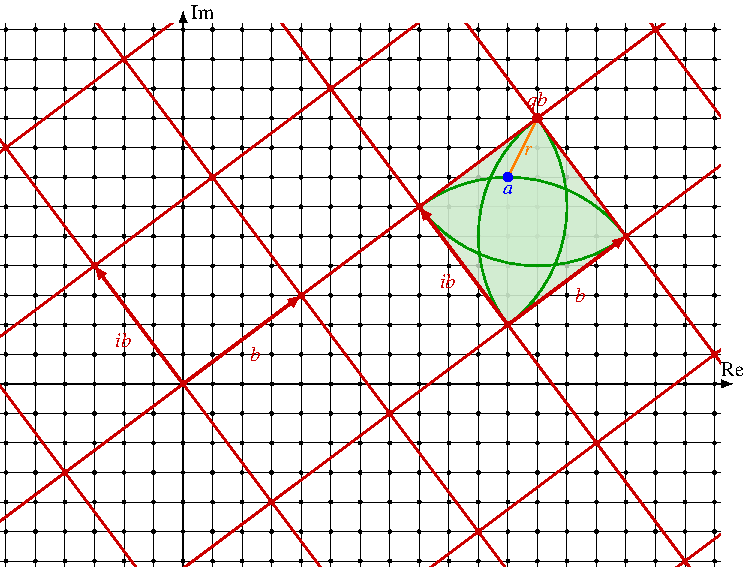
\includegraphics{chapters/060-ratint/images/ggz.pdf}
\caption{Euklidische Eigenschaft des Rings der ganzen gaussschen Zahlen.
Die Vielfachen $\mathbb{Z}[i]b= \{xb+y ib\mid x,y\in\mathbb{Z}\}$
bilden ein quadratisches Gitter ({\color{darkred}rot}). 
Die Zahl $a$ ({\color{blue}blau}) muss in einem der Gitterquadrate
({\color{darkgreen}grün}) liegen, die Seitenkanten $b$ und $ib$ haben.
Da die Kreise mit Radius $|b|$ um die Ecken das ganze Quadrat überdecken,
gibt es eine Ecke, die näher an $a$ ist als $|b|$.
Mit dem $q=x+iy$ dieser Ecke folgt $r=a-qb$ und $|r|<|b|$
bzw.~$d(r) = |r|^2 < |b|^2=d(b)$.
\label{buch:ratint:euklid:fig:ggz}}
\end{figure}
%
Die Menge 
\[
b\mathbb{Z}[i]
=
\{ zb\mid z \in \mathbb{Z}[i] \}
=
\{ xb + iyb \mid x,y\in \mathbb{Z}
\}
\]
bildet ein Gitter in der komplexen Zahlenebene.
Da $b$ und $ib$ senkrecht aufeinander stehende Vektoren sind, 
handelt es sich um ein quadratisches Gitter.
Der Punkt $a$ muss in einem der Gitterquadrate liegen.
Jede Ecke dieses Quadrats wird durch ein $q\in\mathbb{Z}[i]$
beschrieben und kommt als das $q$ in der Eigenschaft~3 eines eukldischen
Rings in Frage.
Die zusätzliche Forderung $d(r)<d(b)$ bedeutet, dass der Punkt $a$
näher als die Kantenlänge des Quadrates bei der ausgewählten Ecke
sein muss.
Da die offenen Kreisscheiben mit Radius $|b|$ die Quadratfläche 
vollständig überdecken, muss es mindestens ein $q\in\mathbb{Z}[i]$
(eine Ecke) geben,
so dass $a-qb=r$ die Bedingung $d(r) < d(b)$ ($|r|<|b|$) erfüllt ist.
\end{enumerate}
Dies zeigt, dass die ganzen gaussschen Zahlen einen euklidischen
Ring bilden.
Es ist daher sinnvoll, vom grössten gemeinsamen Teiler ganzer
gaussscher Zahlen zu sprechen und es ist möglich, diese mit dem
euklidischen Algorithmus zu finden.
\end{beispiel}

Die ganzen gaussschen Zahlen können zum Beispiel dazu verwendet
werden, dann folgenden fermatschen Zweiquadratesatz zu beweisen
\cite[Satz 10.4]{buch:luneburg}.

\begin{satz}[Fermat]
\index{Fermat, Pierre de}%
\index{Satz!von Fermat}%
Ist $p$ eine Primzahl mit $p\equiv 1\mod 4$, dann gibt es ganze
Zahlen $a,b\in\mathbb{Z}$ mit $p=a^2+b^2$.
\end{satz}




%
% 24-koerper.tex -- Körperkoeffizienten
%
% (c) 2026 Prof Dr Andreas Müller
%
\subsection{Polynome mit Koeffizienten in einem beliebigen Körper}
Der euklidische Algorithmus, wie er in
Abschnitt~\ref{buch:ratint:euklid:subsection:polynome}
für Polynome mit Koeffizienten in $\mathbb{Q}$ oder $\mathbb{C}$
vorstellt wurde, ist in keiner Weise auf solche Zahlkörper beschränkt.
Damit die Polynomdivision und damit die Bestimmung des Rests
in jedem Schritt des euklidischen Algorithmus durchgeführt werden kann,
ist nur nötig, dass die Koeffizienten aus einem Körper stammen.
Die Diskussion der Eigenschaften euklidischer Ringe in
Abschnitt~\ref{buch:ratint:euklid:subsection:ringe} hat dies
gezeigt.

Ist $K$ ein Körper, dann ist auch die Menge $F=K(x)$ der rationalen Funktionen
in der Variablen $x$ ein Körper.
$F$ ist ein euklidischer Ring.
Für Polynome mit Koeffizienten in $F$ gilt daher ebenfalls der
euklidische Algorithmus.

Eine Funktion wie
\[
f(z)
=
\frac{2z\log z + 9}{\frac1z-\log z}
\]
kann als rationale Funktion in der Variablen $\vartheta=\log z$
mit Koeffizienten im Körper $\mathbb{Q}(z)$ der rationalen Funktionen
in der Variablen $z$ betrachtet werden.
Zähler und Nenner sind Polynome
\[
2z\vartheta + 9
\qquad\text{und}\qquad
\frac1z -\vartheta
\]
in $\vartheta$ mit rationalen Funktionen als Koeffizienten.
Die Schreibweise
\[
f(z)
=
\frac{2z\vartheta - 9}{\frac1z-\vartheta}
\]
mit $\vartheta$ macht dies deutlich.
Wir werden dies im Kapitel~\ref{chapter:intalg} wiederholt ausnutzen,
um einen Integrationsalgorithmus zu konstruieren.
Wir werden dazu den Grundkörper der rationalen Funktionen in $z$ 
durch weitere Funktionen wie $\vartheta$ erweitern.
Die Erweiterung verlangt nur, dass wir mit rationalen Funktionen
umgehen können müssen.
Zwar ergeben sich zusätzliche Erschwernisse dadurch, dass die Koeffizienten
nicht konstant sind, aber die prinzipielle Vorgehensweise von
Abschnitt~\ref{buch:ratint:bernoulli:subsection:prinzip}
bleibt gültig.





%
% 3-hermite.tex
%
% (c) 2026 Prof Dr Andreas Müller
%
\section{Quadratfreie Faktorisierung und Hermite-Methode
\label{buch:ratint:section:hermite}}
\kopfrechts{Quadratfreie Faktorisierung und die Methode von Hermite}%
Gemäss dem Plan am Ende von Abschnitt~\ref{buch:ratint:section:bernoulli}
ist, ist eine Faktorisierung des Nenners mit sehr speziellen
Teilbarkeitseigenschaften nötig.
Im vorangegangenen Abschnitt wurde mit dem euklidischen Algorithmus
das dazu geeignete Werkzeug bereitgestellt.
Dieses soll jetzt dazu eingesetzt werden, die Faktorisierung zu
finden und den Reduktionsschritt für die Integrale durchzuführen.

%
% Quadratfreie Faktorisierung
%
\subsection{Quadratfreie Faktorisierung}
Die quadratfreie Faktorisierung löst das Problem, den Nenner ohne
Bestimmung der Nullstellen so zu faktorisieren, dass eine
Partialbruchzerlegung möglich wird, mit der die Stammfunktion
bestimmt werden kann.

%
% Mehrfache Nullstellen
%
\subsubsection{Mehrfache Nullstellen}
Sei $q(z) \in \mathbb{C}[z]$ ein Polynom mit einer $n$-fachen Nullstelle
$\alpha$.
Dies bedeutet, dass $q(z)$ in der Form
\[
q(z)
=
(z-\alpha)^n\cdot s(z)
\]
mit einem Polynom $s(z)\in\mathbb{C}[z]$ geschrieben werden kann.
Das Polynom $s(z)$ hat $\alpha$ nicht als Nullstelle, $s(\alpha)\ne 0$,
es ist also nicht durch $z-\alpha$ teilbar.

Nach der Produktregel ist die Ableitung von $q(z)$
\[
q'(z)
=
n
(z-\alpha)^{n-1}
\cdot s(z)
+
(z-\alpha)^n\cdot s'(z)
=
(z-\alpha)^{n-1} 
\cdot \bigl(s(z)+(z-\alpha)\cdot s'(z)\bigr).
\]
Für $z=\alpha$ ist der Klammerfaktor ganz rechts
\[
s(\alpha) + (\alpha-\alpha)\cdot s'(\alpha)
=
s(\alpha)
\ne 0,
\]
der Klammerfaktor hat $\alpha$ nicht als Nullstelle.
Für eine mehrfache Nullstelle ist $n>1$ und es folgt, dass $q'(z)$
die Zahl $\alpha$ als $n-1$-fache Nullstelle hat.

Diese Beobachtung lässt sich auch verallgemeinern.
Hat $q(z)$ einen Faktor $p(z)$, der $n$-fach in $q(z)$ vorkommt,
dann kann man
\[
q(z)
=
p(z)^n\cdot s(z)
\]
schreiben, wobei $s(z)$ nicht durch $p(z)$ teilbar ist.
Die Ableitung von $q'(z)$ ist dann nach der Produktregel
\[
q'(z)
=
n p(z)^{n-1} \cdot s(z) + p(z)^n \cdot s'(z)
=
q(z)^{n-1}\cdot \bigl(ns(z) + p(z) s'(z)\bigr).
\]
Der Faktor auf der rechten Seite ist nicht durch $p(z)$ teilbar,
weil $s(z)$ nicht durch $p(z)$ teilbar ist.
Es folgt, dass $q'(z)$ durch $p(z)^{n-1}$ teilbar ist.

Wenn also $q(z)$ einen mehrfachen vorkommenden Faktor hat,
dann ist dieser Faktor ein gemeinsamer Teiler von $q(z)$
und $q'(z)$.

\begin{beispiel}
Das Polynom 
\begin{align*}
p(z)
&=
z^3 - z^2 - z + 1
&
p(1)&=0
\intertext{hat die Ableitung}
p'(z)
&=
3z^2-2z-1
&
p'(1)
&=
0.
\end{align*}
Die beiden Polynome haben als die gemeinsame Nullstelle $z=1$, somit
muss $(z-1)^2$ ein Faktor von $p(z)$ sein.
Tatsächlich ergibt die Polynomdivision
\[
p(z) : (z-1)^2 = z+1,
\]
woraus sich die Faktorisierung
\[
p(z) = (z-1)^2(z+1)
\]
ergibt.
\end{beispiel}

%
% Quadratfreie Polynome
%
\subsubsection{Quadratfreie Polynome}
Damit $q(z)$ und $q'(z)$ keinen nichtrivialen gemeinsamen Teiler
haben, darf jeder Linearfaktor nur ein einziges Mal vorkommen.
Solche Polynome heissen quadratfrei im Sinne der folgenden
Definition.

\begin{definition}[quadratfrei]
Ein Polynom in $\mathbb{C}[z]$ heisst \emph{quadratfrei}, wenn es
keine mehrfachen Nullstellen hat oder wenn es keine mehrfachen
Faktoren hat.
\index{quadratfrei}%
\end{definition}

Über den komplexen Zahlen zerfällt also ein quadratfreies Polynom
immer in ein Produkt von \emph{verschiedenen} Linearfaktoren.

Wenn ein Polynome $q(z)$ mehrfache Nullstellen hat, dann hat die
Ableitung die gleichen Nullstellen, aber mit einer um $1$ kleineren
Ordnung.
Der grösste gemeinsame Teiler von $q(x()$ und $q'(x)$ besteht
daher aus allen Faktoren, die mehr als einmal vorkommen, mit einer
gegenüber $q(z)$ um $1$ verminderten Vielfachheit.
Im Quotienten
\[
p(z)
=
\frac{q(z)}{\operatorname{ggT}(q(z),q'(z))}
\]
bleiben dann nur noch alle Linearfaktoren genau einmal stehen.

\begin{beispiel}
Das Polynom 
\[
q(z)
=
z^5-z^4-2z^3+2z^2+z-1
\]
hat die Ableitung
\[
q'(z)
=
5z^4-4z^3-6z^2+4z+1.
\]
Der euklidische Algoritmus liefert als grössten gemeinsamen
Teiler das Polynom
\[
g(z)
=
\operatorname{ggT}(q(z), q'(z))
=
z^3-z^2-1+1.
\]
Der Quotient
\[
\frac{q(z)}{g(z)}
=
z^2-1
\]
ist ein quadratfreies Polynom, welches alle Linearfaktoren von $q(z)$
enthält.
Es ist in diesem Fall einfach zu sehen, dass $z^2-1=(z-1)(z+1)$,
d.~h.~die einzigen Nullstellen von $q(x)$ sind $\pm 1$.

Man kann aber die Faktoren auch noch auf etwas systematischere Art
finden.
Dazu berechnet man den grössten gemeinsamen Teiler von $g(z)$ und $g'(z)$,
wegen $g'(z) = 3z^2 -2z -1$ ist
ist
\[
\operatorname{ggT}(g(z),g'(z))
=
z-1
\]
und
\[
\frac{g(z)}{\operatorname{ggT}(g(z),g'(z))}
=
z^2-1.
\]
Daraus kann man schliessen, dass es zwei Linearfaktoren von $q(z)$
gibt.
Einer davon kommt genau zweimal vor, der andere ist $z-1$ und kommt
dreimal vor.
Durch Division $(z^2-1)/(z-1)=z+1$ findet man jetzt, dass $z+1$
der Faktor ist, der genau zweimal enthalten ist.
Wir haben somit die Faktorisierung
\[
q(z)
=
(z+1)^2 (z-1)^3
\]
gefunden.
\end{beispiel}

Das Beispiel zeigt, dass die Suche nach quadratfreien Faktoren
mithilfe des grössten gemeinsamen Teilers manchmal sogar eine
Faktorisierung des Polynoms liefern kann.

%
% Die Aufgabe der Faktorisierung in quadratfreie Faktoren
%
\subsubsection{Die Aufgabe der Faktorisierung in quadratfreie Faktoren}
Ein beliebiges normiertes Polynom $q(z)$ kann einzelne Nullstellen
mehrfach enthalten.
Man kann aber immer noch eine Faktorisierung der Form
\[
q(z)
=
\prod_{k=1}^n
(z-\alpha_k)^{n_k},
\]
wobei alle Nullstellen $\alpha_k$ verschieden sind und $n_k$ ihre
Vielfachheit ist.
Fasst man die Faktoren mit gleicher Vielfachheit zusammen, kann man
zu jeder Vielfachheit $l$ das Polynom
\[
q_l(z) = \prod_{n_k=l} (z-\alpha_k)
\]
bilden.
Da die Faktoren von $q_l(z)$ im Polynom $q(z)$ genau $l$-mal vorkommen,
kann man das Polynom $q(z)$ aus
\[
q(z)
=
q_1(z)
\cdot
q_2(z)^2
\cdot
q_3(z)^3
\cdot
\ldots
\cdot
q_m(z)^m
\]
rekonstruieren.
Nach Konstruktion kann ein Linearfaktor nur immer in genau einem
der Faktoren $q_l(z)$ vorkommen, die Faktoren sind also paarweise
teilerfremd.

\begin{definition}[quadratfreie Faktorisierung]
\index{quadratfreie Faktorisierung}%
\index{Faktorisierung, quadratfrei}%
Die \emph{quadratfreie Faktorisierung} eines Polynoms $q(z)$ ist eine
Faktorisierung der Form
\[
q(z)
=
a
\prod_{l=1}^m q_l(z)^l
\]
mit teilerfremden Faktoren.
\end{definition}

Die Bestimmung der quadratfreien Faktorisierung aus der Zerlegung
in Linearfaktoren zeigt zwar, dass es eine solche Faktorisierung
gibt, ist aber kein praktikabler Weg, sie algorithmisch zu bestimmen.
daher soll in diesem Abschnitt die folgende Aufgabe gelöst werden.

\begin{aufgabe}
Formuliere einen Algorithmus, der zu einem beliebigen rationalen Polynom
$q(z)\in\mathbb{Q}[z]$ die quadratfreie Faktorisierung findet.
\end{aufgabe}

%
% Berechnung der quadratfreien Faktorisierung
%
\subsubsection{Berechnung der quadratfreien Faktorisierung}
Aus dem Beispiel lesen wir ab, dass der grösste gemeinsame
Teiler $g(z)=\operatorname{ggT}\bigl(q(z),q'(z)\bigr)$ von $q(z)$
und $q'(z)$ alle mehrfachen Faktoren enthält und der Quotient
$q(z)/g(z)$ alle Linearfaktoren genau einmal.
Diese Eigenschaft soll jetzt dazu verwendet werden, die Faktoren
$q_l(z)$ zu finden.
Dazu konstruieren wir zunächst zwei Folgen $g_k(z)$ und $p_k(z)$
wie folgt.
Das Polynom $g_0(z)$ ist $g_0(z)=q(z)$.
Die Polynome $g_k(z)$ und $p_k(z)$ mit $k>0$ sind rekursiv definiert
durch
\begin{align*}
g_{k+1}(z) &= \operatorname{ggT}\bigl(g_k(z),g'_k(z)\bigr)
&&\text{und}&
p_{k+1}(z) &= \frac{g_k(z)}{g_{k+1}(z)}.
\end{align*}
Nach Konstruktion sind die Polynom $p_k(z)$ alle quadratfrei.
Sie enthalten alle Linearfaktoren von $g_k(z)$.
Nach Konstruktion ist $g_{k+1}(z)$ immer ein echter Teiler von $g_k(z)$.
Der Grad nimmt in jedem Schritt ab.
Die Konstruktion bricht daher nach endlich vielen Schritten ab.

In jedem Iterationsschritt nimmt der Exponent der in $g_k(z)$
vertretenen Linearfaktoren um $1$ ab.
Das Ende $g_k(z)=1$ wird also genau in dem Moment erreicht, 
in dem der grösste Exponent auf $1$ reduziert worden ist.
Somit ist $k$ der grösste Exponent eines Linearfaktors.

Die Polynome $p_k(z)$ enthalten alle Linearfaktoren, die
mindestens $k$ mal in $q(z)$ aufreten.
Es folgt, dass $p_{k+1}(z)$ ein Teiler von $p_k(z)$ ist und dass
der Quotient $p_k(z)/p_{k+1}(z)$ aus den Faktoren besteht, die 
genau $k$-mal in $q(z)$ vorkommen.
Dies ist genau, was die Polynome $q_l(z)$ definiert.
Dies beweist den folgenden Satz.

\begin{satz}[quadratfreie Faktorisierung]
\index{Satz!quadratfreie Faktorisierung}%
Sei $q(z)\in K[z]$ ein normiertes Polynom.
Setze $q_0(z)=q(z)$ und bilde rekursiv die Folgen
\begin{align*}
g_k(z) &= \operatorname{ggT}\bigl(g_{k-1}(z),g_{k-1}'(z)\bigr),
&
p_k(z) &= \frac{g_{k-1}(z)}{g_k(z)},
&
q_k(z) &= \frac{p_k(z)}{p_{k+1}(z)}.
\end{align*}
Sei $m$ dasjenige $k$, für das $p_k(z)=1$ ist.
Dann ist
\[
q(z)
=
\prod_{l=1}^m q_l(z)^l
\]
die quadratfreie Faktorisierung.
\end{satz}

\begin{beispiel}
Wir betrachten das Polynom
\begin{align*}
q(z)
&=
z^9+z^8-5z^7-5z^6+9z^5+9z^4-7z^3-7z^2+2z+2
\intertext{mit der Ableitung}
q'(z)
&=
9z^8+8z^7-35z^6-30z^5+45z^4+36z^3-21z^2-14z+2
\end{align*}
Die Polynome $g_k(z)$, $p_k(z)$ und $q_l(z)$ sind
\begin{align*}
g_1(z)
&=
z^5+z^4-2z^3-2z^2+z+1,
&
p_1(z)
&=
z^4-3z^2+2,
&
q_1(z)
&=
z^2-2,
\\
g_2(z)
&=
z^3+z^2-z-1,
&
p_2(z)
&=
z^2-1,
&
q_2(z)
&=
1,
\\
g_3(z)
&=
z+1
&
p_3(z)
&=
z^2-1,
&
q_3(z)
&=
z-1,
\\
g_4(z)
&=
1,
&
p_4(z)
&=
z+1,
&
q_4(z)
&=
z+1,
\\
g_5(z)
&=
1,
&
p_5(z)
&=
1.
&
&
\end{align*}
Tatsächlich kann man nachrechnen, dass
\[
q(z)
=
(z^2-2)(z-1)^3(z+1)^4
\]
ist.
Man beachte aber, dass diese Faktorisierung mit $z^2-2$ auch einen Faktor
enthält, der kein Linearfaktor ist.
Da $z^2-2 = (z+\!\sqrt{2})(z-\!\sqrt{2})$, gibt es über $\mathbb{Q}$
keine Faktorisierung in Linearfaktoren.
\end{beispiel}

\begin{beispiel}
\label{buch:ratint:hermite:bsp:qf2}
Man finde die quadratfreie Faktorisierung des Polynoms
\[
q(z) = 9z^6 + 6z^5 - 65z^4 + 20z^3 + 135z^2 - 154z + 49
\]
mit der Ableitung
\[
q'(z) = 54z^5+30z^4-260z^3+60z^2+270z-154.
\]
Die Polynome $g_k(z)$, $p_k(z)$ und $q_l(z)$ sind
\begin{align*}
g_1(z)
&= 
3z^4-2z^3-12z^2+18z-7,
&
p_1(z)
&=
3z^2+4z-7,
&
q_1(z)
&=
1,
\\
g_2(z)
&=
z^2-2z+1,
&
p_2(z)
&=
3z^2+4z-7,
&
q_2(z)
&=
3z+7,
\\
g_3(z)
&=
z-1,
&
p_3(z)
&=
z-1,
&
q_3(z)
&=
1,
\\
g_4(z)
&=
1,
&
p_4(z)
&=
z-1,
&
q_4(z)
&=
z-1,
\\
g_5(z)
&=
1,
&
p_5(z)
&=
1.
&&
\end{align*}
Daraus liest man die quadratfreie Faktorisierung
\[
q(z)
=
(3z+7)^2(z-1)^4
\]
ab.
\end{beispiel}

%
% Reduktion des Integrals
%
\subsection{Reduktion des Integrals}
Mit dem Werkzeug der quadratfreien Faktorisierung lässen sich jetzt
die für den rationalen Teil des Integrals nötigen Schritte des Plans
vom Ende von Abschnitt~\ref{buch:ratint:section:bernoulli} durchführen.
Zu diesem Zwck muss erst eine Partialbruchzerlegung gefunden werden.
Anschliessend müssen die einzelnen Terme der Partialbruchzerlegung
integriert werden.

%
% Partialbruchzerlegung zur quadratfreien Faktorisierung
%
\subsubsection{Partialbruchzerlegung zur quadratfreien Faktorisierung}
Der wesentliche Schritt zur Konstruktion der Partialbruchzerlegung
ist der folgende Satz.

\begin{satz}
Sei 
\[
f(z)
=
\frac{p(z)}{q(z)^m r(z)},
\]
wobei $q(z)$ teilerfremd zu $r(z)$ ist.
Dann gibt es 
\[
f(z)
=
f_0(z)
+
\frac{s(z)}{r(z)}
+
\sum_{k=1}^m \frac{t_k(z)}{q(z)^k},
\]
wobei $f_0(z)$ ein Polynom ist, $s(z)$ ein Polynom mit Grad
$\deg s(z)<\deg r(z)$ und die Polynome $t_k(z)$ Grad $\deg t_k(z)<\deg q(z)$
haben.
\end{satz}

\begin{proof}
Da $q(z)$ und $r(z)$ teilerfremd sind, sind auch $q(z)^m$ und $r(z)$
teilerfremd.
Daher gibt es $s(z)$ und $t(z)$ mit
\begin{equation}
p(z)
=
s(z)q(z)^m + t(z)r(z).
\label{buch:ratint:hermite:eqn:p=sq+tr}
\end{equation}
Einsetzen in den Bruch ergibt
\begin{align}
f(z)
&=
\frac{p(z)}{q(z)^m r(z)}
=
\frac{s(z)q(z)^m + t(z)r(z)}{q(z)^mr(z)}
=
\frac{s(z)}{r(z)}
+
\frac{t(z)}{q(z)^m}.
\label{buch:ratint:hermite:eqn:srtq}
\end{align}
Falls der Zähler einen Grad mindestens so gross wie der Nenner
hat, kann durch Division des Zählers mit Rest das Polynom $f_0(z)$
abgespaltet werden.

Es muss jetzt nur noch gezeigt werden, dass der zweite Bruch in
\eqref{buch:ratint:hermite:eqn:srtq}
in eine Summe der verlangten Art umgeformt werden kann.
Dazu schreibt man den Zähler mithilfe der Polynomdivision als
\begin{equation*}
t(z)
=
a_m(z) q(z) + t_{m}(z)
\end{equation*}
mit $\deg b(z) < \deg q(z)$.
Dann wird
\begin{align*}
\frac{t(z)}{q(z)^m}
&=
\frac{a(z)q(z)+b(z)}{q(z)^m}
=
\frac{a(z)}{q(z)^{m-1}}
+
\frac{b(z)}{q(z)^m}.
\intertext{Durch wiederholte Anwendung dieser Beobachtung auf
den neuen Zähler $a_m(z) = a_{m-1}(z)q(z)+t_{m-1}(z)$
wird daraus eine Summe der Form}
&=
\frac{t_1(z)}{q(z)}
+
\frac{t_2(z)}{q(z)^2}
+
\ldots
+
\frac{t_m(z)}{q(z)^m}.
\end{align*}
Damit ist der Satz vollständig bewiesen.
\end{proof}

Durch Anwendung auf eine Faktorisierung von $r(z)$ kann schrittweise
die Partialbruchzerlegung mit den Teilnennern $q_l(z)^k$, $k\le l$
für alle $l$ gefunden werden.
Man beachte, dass dazu wieder nur die Polynomdivision
und für die Identität 
\eqref{buch:ratint:hermite:eqn:p=sq+tr}
der euklidische Algorithmus benötigt werden.
Beide können für Polynome in einer beliebigen Körpererweiterung
für den Koeffizientenkörper durchgeführt werden.

\begin{beispiel}
\label{buch:ratint:hermite:bsp:partialbruch}
Man finde die Partialbruchzerlegung von
\[
\frac{r(z)}{q(z)}
\quad\text{mit}\quad
\left\{\;
\renewcommand{\arraycolsep}{2pt}
\begin{array}{rcl}
r(z) &=& 6651z^4 + 3969z^2 - 37338z + 21854 \\
q(z) &=& 9z^6 + 6z^5 - 65z^4 + 20z^3 + 135z^2 - 154z + 49.
\end{array}\right.
\]
Man verwendet dafür die quadratfreie Faktorisierung
\[
q(z)
=
(z-1)^4(3z+7)^2,
\]
die in Beispiel~\ref{buch:ratint:hermite:bsp:qf2} gefunden worden war.
Zunächst sind die beiden Faktoren $(z-1)^4$ und $(3z+7)^2$
teilerfremd, so dass es Polynome $s(z)$ und $t(z)$ gibt derart,
dass
\begin{align*}
r(z) &= s(z)(z-1)^4 + t(z) (3z+7)^2
\intertext{nämlich}
s(z) &=
	\frac{1}{50000}(3214890^5 z + 10180485 z^4 + 1928934 z^3 - 12037977 z^2
	- 46842138 z\\
     &\phantom{50000}\qquad + 33633306)
\\
t(z) &=
	\frac{1}{50000}(357210 z^7 - 1964655 z^6 + 5056506 z^5 - 9737280 z^4
	+ 15174810 z^3\\
     &\phantom{50000}\qquad - 37747395 z^2  + 52924410 z - 21613606),
\end{align*}
wie man mit dem erweiterten euklidischen Algorithmus finden kann.
Bildet man jetzt die Quotienten $s(z)/q(z)$ und $t(z)/q(z)$, heben sich die
polynomiellen Teile weg und es bleibt
\index{polynomieller Teil}%
\[
\frac{r(z)}{q(z)}
=
\frac{2646}{(3z+7)^2}
+
\frac{441z^2-882z+392}{(z-1)^4}.
\]
Der zweite Term hat noch nicht die von der Partialbruchzerlegung verlangte
Form.
Dies wird erreicht, indem man den Zähler wiederholt mit Rest durch $z-1$
dividiert:
\[
\left.
\begin{aligned}
441z^2-882z+392 &= (441z-441) (z-1 ) - 49 \\
441z-441 &= 441 (z-1) + 0
\end{aligned}\right\}
\Rightarrow
441z^2-882z+392 = 441 (z-1)^2 - 49.
\]
Daraus ergeben sich jetzt die Partialbrüche zum Teilnenner $z-1$ als
\[
\frac{t(z)}{(z-1)^4}
=
\frac{441}{(z-1)^2} - \frac{49}{(z-1)^4}.
\]
Insgesamt ist also
\[
\frac{r(z)}{q(z)}
=
\frac{2646}{(3z+7)^2}
+
\frac{441}{(z-1)^2} - \frac{49}{(z-1)^4}
\]
die gesuchte Partialbruchzerlegung.
\end{beispiel}


%
% Integration des rationalen Teils
%
\subsubsection{Integration des rationalen Teils}
Ganz analog der Vorgehensweise in der Methode von Bernoulli im
Abschnitt~\ref{buch:ratint:section:bernoulli} können auch die
Integranden mit Potenzen quadratfreier Polynome $q(z)$ im Nenner
auf den Nenner $q(z)$ reduziert werden.

\begin{satz}[Hermite]
\label{buch:ratint:hermite:satz:reduktion}
\index{Satz!von Hermite}%
Sei $q(z)$ ein quadratfreies Polynom und $p(z)$ ein beliebiges
Polynom von kleinerem Grad $\deg q(z)<\deg p(z)$.
Dann gibt es Polynome $s(z)$ und $t(z)$ Polynome mit
\begin{equation}
s(z)\cdot q(z)
+
t(z)\cdot q'(z)
=
p(z),
\label{buch:ratint:hermite:ggtsz}
\end{equation}
für die zudem
\begin{align}
\int
\frac{p(z)}{q(z)^m}
\,dz
&=
\int
\frac{s(z)+t'(z)/(m-1)}{q(z)^{m-1}}
\,dz
+
\frac{t(z)}{(1-m)q(z)^{m-1}}
\label{buch:rating:hermite:satz:hermite:eqn:int}
\end{align}
wird.
\end{satz}

\begin{proof}
Da $q(z)$ quadratfrei ist sind  $q(z)$ und $q'(z)$ teilerfremd.
Nach dem euklidischen Algorithmus für Polynome gibt es daher
Polynome $s(z)$ und $t(z)$ derart, dass \eqref{buch:ratint:hermite:ggtsz}
gilt.
Einsetzen ins Integral ergibt
\begin{align*}
\int
\frac{p(z)}{q(z)^m}
\,dz
&=
\int
\frac{s(z)\cdot q(z)+t(z)\cdot q'(z)}{q(z)^m}
\,dz
\\
&=
\int
\frac{s(z)}{q(z)^{m-1}}
\,dz
+
\int
t(z)
\cdot
\frac{q'(z)}{q(z)^m}
\,dz
\intertext{Auf das zweite Integral kann partielle Integration
angewendet werden.
Das Polynom $p(z)$  wird abgeleitet während der Bruch
$q'(z)/q(z)^m$ integriert wird.
So entsteht}
&=
\int
\frac{s(z)}{q(z)^{m-1}}
\,dz
+
t(z)
\frac{1}{(1-m)q(z)^{m-1}}
-
\int
\frac{t'(z)}{(1-m)q(z)^{m-1}}
\,dz
\\
&=
\int
\frac{s(z)+t'(z)/(m-1)}{q(z)^{m-1}}
\,dz
+
t(z)
\frac{1}{(1-m)q(z)^{m-1}}.
\end{align*}
Damit ist der Satz bewiesen.
\end{proof}

Durch wiederholte Anwendung des
Satzes~\ref{buch:ratint:hermite:satz:reduktion}
kann man die Potenz des Nenners immer weiter reduzieren, bis
nur noch das Integral
\[
\int
\frac{p(z)}{q(z)}
\,dz
\]
bestimmt werden muss, wobei $p(z)$ und $q(z)$ teilerfremd sind,
$\deg p(z)<\deg q(z)$ und $q(z)$ quadratfrei.
Dieser Teil des Integrationsproblems heisst auch der 
\emph{logarithmische Teil} des Integrals.
\index{logarithmischer Teil}%
Die Methode von Hermite vermeidet eine vollständige Faktorisierung
und ersetzt sie durch eine quadratfreie Faktorisierung.
Sie erreicht aber auch nur eine Reduktion auf quadratfreie Nenner.
Für die vollständig Berechnung der Stammfunktion ist nach der Methode
von Bernoulli weiterhin eine Faktorisierung der quadratfreien Faktoren
sein.
Dies wird aber potentiell dadurch vereinfacht, dass alle Nullstellen
eines quadratfreien Polynoms einfach sind.

\begin{beispiel}
Man finde die Stammfunktion
\begin{align*}
F(z)
&=
\int
\frac{p(z)}{q(z)}\,dz
\\
&=
\int
\frac{
441z^7 + 780z^6 - 2861z^5 + 4085z^4 + 7695z^3 + 3713z^2 - 43253z + 24500
}{
9z^6 + 6z^5 - 65z^4 + 20z^3 + 135z^2 - 154z + 49
}
\,dz
\end{align*}
mit den Polynomen
\begin{align*}
p(z)
&=
441z^7 + 780z^6 - 2861z^5 + 4085z^4 + 7695z^3 + 3713z^2 - 43253z + 24500
\\
q(z)
&=
9z^6 + 6z^5 - 65z^4 + 20z^3 + 135z^2 - 154z + 49.
\end{align*}
Zunächst muss man den Bruch mit Reset dividieren und erhält
\[
F(z)
=
\int 49z + 54\,dz
+
\int
\frac{6651z^4 + 3969z^2 - 37338z + 21854}{q(z)}\,dz,
\]
wobei wir den Zähler im zweiten Integral mit $r(z)$ bezeichnen wollen.
Für die weitere Vereinfachung des zweiten Integrals wird jetzt die
quadratfreie Faktorisierung von $q(z)$ benötigt.
Sie ist
\[
q(z)
=
(z-1)^4(3z+7)^2.
\]
In diesem Fall hat die quadratfreie Faktorisierung eine vollständige
Faktorisierung in Linearfaktoren geliefert.
Damit kann jetzt auch die Partialbruchzerlegung gefunden werden,
wie dies in Beispiel~\ref{buch:ratint:hermite:bsp:partialbruch}
bereits geschehen ist.
Sie ist
\begin{equation}
\frac{r(z)}{q(z)}
=
\frac{294}{(z+\frac{7}{3})^2}
+
\frac{441}{(z-1)^2}
-
\frac{49}{(z-1)^4}.
\label{buch:ratint:hermite:bps:hermite:pf}
\end{equation}
Für die einzelnen Summanden ist jetzt noch die Reduktion nach der Methode
von Hermite von Satz~\ref{buch:ratint:hermite:satz:reduktion} durchzuführen.

Für den ersten Term müssen mit dem euklidischen Algorithmus
$s(z)$ und $t(z)$ gefunden werden derart, dass
\[
s(z)(z+{\textstyle\frac{3}{7}}) + t(z)(z+{\textstyle\frac{3}{7}})
=
s(z)(z+{\textstyle\frac{3}{7}}) + t(z) = 294
\]
gilt, nämlich $s(z)=0$ und $t(z)=294$.
Daraus folgt das Integral für den ersten Term als
\[
\int \frac{294}{(z+\frac37)^2}
=
-\frac{294}{z+{\textstyle\frac37}},
\]
wie man auch von der bekannten Integrationsformel erwartet hätte.

Für den zweiten Term muss man $s(z)$ und $t(z)$ finden derart, dass
\[
s(z)(z-1) + t(z)(z-1)' = s(z)(z-1) + t(z) = 441
\]
gilt.
Der euklidische Algorithmus liefert $s(z)=0$ und $t(z)=441$ und daher
\[
\int \frac{441}{(z-1)^2}\,dz
=
-
\frac{441}{z-1}.
\]
Ebenso funktioniert die Methode für den dritten Term.
Man muss $s(z)$ und $t(z)$ finden derart, dass
\[
s(z)(z-1) + t(z)(z-1)' = s(z)(z-1) + t(z) = -49
\]
gilt.
Es folgt $s(z)=0$ und $t(z)=-49$ und damit 
\[
\int \frac{-49}{(z-1)^4} \,dz
=
\frac{49}{3(z-1)^3}.
\]
Damit ist das gesuchte Integral
\[
F(z)
=
-
\frac{294}{z+\frac{3}{7}}
-
\frac{441}{z-1}
+
\frac{49}{3(z-1)^3}
\]
gefunden.
\end{beispiel}

\begin{beispiel}
Man bestimme das Integral
\[
F(z)
=
\int \frac{p(z)}{q(z)} \,dz
=
\int \frac{z+1}{(z^2+1)^3} \,dz.
\]
Der Nenner liegt bereits in der quadratfreien Faktorisierung mit dem
Faktor $q(z)=z^2+1$ vor, somit hat der Integrand bereits die Form der
Partialbruchzerlegung, es bleibt nur noch, die Reduktion nach Hermite 
mit $m=3$ zu finden.
Dazu werden zunächst $s(z)$ und $t(z)$ bestimmt mit
\[
s(z)q(z) + t(z)q'(z) = z+1,
\]
man findet $s(z)=z+1$ und $t(z)=-\frac12(z^2+z)$.
Einsetzen in die Formel~\eqref{buch:rating:hermite:satz:hermite:eqn:int}
ergibt
\begin{align}
\int
\frac{z+1}{(z+1)^3}
\,dz
&=
\int \frac{2z}{3(z^2+1)^2} \,dz
+
\frac{z^2+z}{4z^4+8z^2+4}.
\label{buch:ratint:hermite:bsp:hermite2:eqn:i3}
\end{align}
Der Prozess muss jetzt für das verbleibende Integral auf der rechten
Seite wiederholt werden.
Diesmal findet man
\[
s(z)=\frac{2z+3}{4}
\qquad\text{ und }\qquad
t(z)=-\frac{2z^2+3}{8}
\]
und nach Einsetzen
\begin{align}
\int \frac{2z}{3(z^2+1)^2} \,dz
&=
\int \frac{\frac{3}{8}}{z^2+1}\,dz
+
\frac{2z^2+3z}{8z^2+8}.
\label{buch:ratint:hermite:bsp:hermite2:eqn:i2}
\end{align}
Kombiniert man
\eqref{buch:ratint:hermite:bsp:hermite2:eqn:i3}
und
\eqref{buch:ratint:hermite:bsp:hermite2:eqn:i2}
findet man
\begin{align*}
\int
\frac{z+1}{(z+1)^3}\,dz
&=
\frac38 \int \frac{1}{z^2+1}\,dz
+
\frac{2z^4+3z^3+4z^2+5z}{8z^4+16z^2+8}
\\
&=
\arctan z
+ 
\frac{3z^3+5z-2}{8z^4+16z^2+8}
+\frac14.
\end{align*}
Der Term $\frac14$ auf der echten Seite ist entstanden durch Division
des Zählers mit Rest durch den Nenner.
Er kann in der Integrationskonstanten absorbiert werden.
\end{beispiel}

%\input{chapters/060-ratint/33-horowitz.tex}

%
% 4-rothsteintrager.tex
%
% (c) 2026 Prof Dr Andreas Müller
%
\section{Die Methode von Rothstein-Trager
\label{buch:ratint:section:rothsteintrager}}
\kopfrechts{Die Methode von Rothstein-Trager}%
Die Methode von Rothstein-Trager ermöglicht, auch den logarithmischen
Teil
\begin{equation}
I
=
\int
\frac{p(z)}{q(z)}
\,dz
\label{buch:ratint:rothsteintrager:eqn:integral}
\end{equation}
für einen quadratfreien Nenner $q(z)$ und einen dazu teilerfremden
Zähler $p(z)$ mit $\deg p(z)<\deg q(z)$ zu berechnen.

%
% Residuen und die Form des Integrals
%
\subsection{Residuen und die Form des Integrals
\label{buch:ratint:rothsteintrager:subsection:residuen}}
In den komplexen Zahlen lässt sich der quadratfreie Nenner $q(z)$ von
\eqref{buch:ratint:rothsteintrager:eqn:integral}
in ein Produkt verschiedener Linearfaktoren
\begin{equation}
q(z)
=
(z-\alpha_1)\cdots(z-\alpha_n)
\label{buch:ratint:rothsteintrager:eqn:faktorisierung}
\end{equation}
zerlegen.
Da die Nullstellen alle verschieden sind, hat die Partialbruchzerlegung
des Integranden die Form
\begin{equation}
\frac{p(z)}{q(z)}
=
\frac{A_1}{z-\alpha_1}
+
\ldots
+
\frac{A_n}{z-\alpha_n}.
\label{buch:ratint:rothsteintrager:eqn:integrand}
\end{equation}
In dieser Form lässt sich das Integral jedoch sofort angeben, es ist
\begin{equation}
\int
\frac{p(z)}{q(z)}
\,dz
=
A_1\log(z-\alpha_1)
+
\ldots
+
A_n\log(z-\alpha_n).
\label{buch:ratint:rothsteintrager:eqn:integralform}
\end{equation}
Der Ausdruck kann noch etwas vereinfacht werden, wenn zwei der
Koeffizienten gleich sind.
Ist nämlich $A_k=A_l$, dann können die beiden Summanden in
$A_k\log\bigl((z-\alpha_k)(z-\alpha_k)\bigr)$
zusammengefasst werden.
Für entgegengesetzte Koeffizienten $A_k=-A_l$ folgt entsprechend
\[
A_k\log \frac{z-\alpha_k}{z-\alpha_l}.
\]
Diese Form tritt zum Beispiel bei der Integration reeller Funktionen
auf, wo die Nullstellen des Nenners paarweise konjugiert komplex sind.

Wenn die Faktorisierung
\eqref{buch:ratint:rothsteintrager:eqn:faktorisierung}
von $q(z)$ bekannt ist, ist das Integrationsproblem an dieser
Stelle gelöst.
Wie früher bereits dargelegt wurde, kann man jedoch nicht davon
ausgehen, dass das Faktorisierungsproblem gelöst werden kann.
Es müssen also alternative Methoden gesucht werden, die ohne die 
die Faktorisierung auskommen.

%
% Die Koeffizienten A_k und Residuen
%
\subsubsection{Die Koeffizienten $A_k$ und Residuen}
Die Form 
\eqref{buch:ratint:rothsteintrager:eqn:integrand}
des Integranden des logarithmischen Teils zeigt, dass er isolierte
Singularitäten hat und daher um jede Singularität in eine Laurent-Reihe
entwickelt werden kann.
\index{Singularitat@Singularität}%
Man kann sogar sagen, dass die Singularitäten Pole erster Ordnung
sein müssen.

Sei jetzt $\alpha$ eine dieser Pole, dann kann der Integrand
in eine Laurent-Reihe
\index{Laurent-Reihe}%
\[
\frac{p(z)}{q(z)}
=
\frac{b_1}{z-\alpha}
+
a_0+a_1(z-\alpha) + a_2(z-\alpha)^2+\ldots
\]
um den Punkt $\alpha$ entwickelt werden.
Gliedweise Integration der Reihe ergibt in einer Umgebung von $\alpha$
\[
\int
\frac{p(z)}{q(z)}
\,dz
=
b_1\log(z-\alpha)
+
a_0(z-\alpha) + \frac{a_1}{2}(z-\alpha)^2 + \frac{a_2}{3}(z-\alpha)^3
+\ldots
\]
Durch Vergleich mit
\eqref{buch:ratint:rothsteintrager:eqn:integralform}
folgt, dass die gesuchten Koeffizienten $A_k$ die Residuen
des Integranden an den Nullstellen von $q(z)$ sein müssen.
\index{Residuum}%
Diese Koeffizienten lassen sich aber direkt aus den Polynomen 
$p(z)$ und $q(z)$ berechnen.

\begin{satz}
\label{buch:ratint:rothsteintrager:satz:residuum}
Sind $p(z)$ und $q(z)$ teilerfremd und $q(z)$ quadratfrei und
$\alpha$ eine Nullstelle des Nenners.
Dann ist das Residuum von $p(z)/q(z)$ an der Stelle $\alpha$
\[
A
=
\operatorname{res}\biggl(\alpha;\frac{p(z)}{q(z)}\biggr)
=
\frac{p(\alpha)}{q'(\alpha)}.
\]
\index{resz0f@$\operatorname{res}(z_0;f)$}%
\end{satz}

Der Satz ist eine direkte Folge des
Satzes~\ref{buch:analytisch:laurent:residuum:satz}.


%
% Der Satz von Rothstein-Trager
%
\subsection{Der Satz von Rothstein-Trager}
Die Form des logarithmischen Teils des Integrals ist zwar bekannt,
und der Satz~\ref{buch:ratint:rothsteintrager:satz:residuum}
ermöglicht eine direkte Berechnung des Koeffizienten, sobald
die Nullstellen bekannt sind, aber genau die Bestimmung der
Nullstellen war ja der Punkt, warum die Methode von Bernoulli
als unzureichend erkannt wurde.
Dies ändert der folgende Satz von Rothstein-Trager.

\begin{satz}[Rothstein-Trager]
\label{buch:ratint:rothsteintrager:satz:rothsteintrager}
\index{Rothstein, Michael}%
\index{Trager, Barry M.}%
Ist $p(z)$ teilerfremd zum normierten, quadratfreien Polynom $q(z)$ mit
$\deg p(z)<\deg q(z)$, dann ist
\begin{equation}
\int
\frac{p(z)}{q(z)}
\,dz
=
\sum_{k=1}^m c_k \log v_k(z),
\label{buch:ratint:rothsteintrager:eqn:rtintegral}
\end{equation}
wobei die $c_k$ die verschiedenen, möglicherweise komplexen Zahlen $c$ sind
derart, dass $p(z)-cq'(z)$ und $q(z)$ einen nichttrivialen gemeinsamen
Teiler haben.
Die zugehörigen $v_k(z)$ sind
\[
v_k(z)
=
\operatorname{ggT}\bigl(p(z)-c_kq'(z),q(z)\bigr).
\]
Sie sind normiert, teilerfremd und quadratfrei.
\end{satz}

Aus der Methode von Bernoulli ist bekannt, dass die Stammfunktion tatsächlich
\index{Bernoulli!Methode von}%
die Form~\eqref{buch:ratint:rothsteintrager:eqn:rtintegral} hat.
Danach sind die $v_k(z)$ verschiedene Linearfaktoren, deren Produkt
\[
q(z)
=
\prod_{k=1}^m v_k(z)
\]
ist.
Falls zwei Faktoren $v_i(z)$ und $v_k(z)$ den gleichen Koeffizienten
$c=c_i=c_k$ haben, können die beiden Terme zu einem Term $v(z)$
zusammengefasst werden mit $v(z) = v_i(z)v_k(z)$.
Es ist nämlich
\[
cv(z)
=
c\log \bigl(v_i(z)v_k(z)\bigr)
=
c(\log v_i(z) + \log v_k(z))
=
c_i \log v_i(z) + c_k\log v_k(z).
\]
Man darf also sogar davon ausgehen, dass die $c_k$ alle verschieden
sind und die $v_k(z)$ Produkte von verschiedenen Linearfaktoren.
Somit haben die $v_k(z)$ nur einfache Nullstellen, sie sind also
alle quadratfrei.

\begin{proof}
Nach der Vorbemerkung muss noch gezeigt werden, dass die Konstanten
$c_k$ und die Polynome $v_k(z)$ auf die genannte Art gefunden werden
können.
Wir nehmen dazu an, dass die Stammfunktion die Form 
\eqref{buch:ratint:rothsteintrager:eqn:rtintegral} hat
und schreiben
\begin{align*}
u_k(z) &= \prod_{\scriptstyle i=1\atop \scriptstyle i\ne k}^m v_i(z)
&&\text{und}&
v(z)   &= \prod_{i=1}^m v_i(z).
\end{align*}
Die Ableitung von \eqref{buch:ratint:rothsteintrager:eqn:rtintegral} ist
\[
\frac{p(z)}{q(z)}
=
\sum_{k=1}^m c_k \frac{v'_k(z)}{v_k(z)}.
\]
Durch Multiplizieren mit $q(z)$ und allen $v_i(z)$, $i=1,\dots,m$,
erhalten wir
\begin{equation}
p(z)\prod_{i=1}^m v_i(z)
=
\sum_{k=1}^m
c_k
q(z)
v'_k(z)
\prod_{\scriptstyle i=1 \atop \scriptstyle i\ne k}^m v_i(z)
=
\sum_{k=1}^m
c_k
q(z)
v'_k(z)
u_k(z).
\label{buch:ratint:rothsteintrager:eqn:produkt}
\end{equation}

Für den Beweis gehen wir in den folgenden Schritten vor:
\begin{enumerate}
\item Schritt:
$q(z)$ teilt das Produkt $v(z)$ aller $v_i(z)$.
Die rechte Seite von \eqref{buch:ratint:rothsteintrager:eqn:produkt}
enthält den Faktor $q(z)$, also muss auch die linke Seite durch $q(z)$
teilbar sein.
Da $p(z)$ und $q(z)$ teilerfremd sind, muss $q(z)$ ein Teiler des
Produktes auf der linken Seite von
\eqref{buch:ratint:rothsteintrager:eqn:produkt} sein.

\item Schritt:
Jeder Faktor $v_i(z)$ teilt $q(z)$.
$v_i(z)$ ist ein Faktor der linken Seite von
\eqref{buch:ratint:rothsteintrager:eqn:produkt}
und jedes Faktors $c_kq(z)v'_k(z)u_k(z)$ der rechten Seite ausser
im Fall $k=i$.
Daher muss $v_i(z)$ ein Teiler von $c_iq(z)v'_i(z)u_i(z)$ sein.
Die Polynome $v_i(z)$ und $u_i(z)$ sind teilerfremd und weil $v_i(z)$
quadratfrei sind auch $v_i(z)$ und $v'_i(z)$.
Somit muss $v_i(z)$ ein Teiler von $q(z)$ sein.

\item Schritt:
Jeder Faktor $v_i(z)$ ein Teiler von $q(z)$, also ist auch
das Produkt $v(z)$ ein Teiler von $q(z)$.
Da sowohl $v(z)$ als auch $q(z)$ normierte Polynome sind, folgt aus
$v(z)\mid q(z)$ und $q(z)\mid v(z)$, dass $v(z)=q(z)$.

\item Schritt: wegen $v(z)=q(z)$ kann man jetzt beide Seiten von
\eqref{buch:ratint:rothsteintrager:eqn:produkt}
durch $q(z)$ teilen und erhält
\begin{equation}
p(z)
=
\sum_{i=1}^m
c_i
v'_i(z)
u_i(z).
\label{buch:ratint:rothsteintrager:eqn:produkt2}
\end{equation}

\item Schritt:
Die Gleichung
\eqref{buch:ratint:rothsteintrager:eqn:produkt2} kann auch als
\[
p(z)-c_k v'_k(z) u_k(z)
=
\sum_{\scriptstyle i=1\atop \scriptstyle i\ne k}^m c_iv'_i(z) u_i(z)
\]
geschrieben werden.
Ein nichttrivialer Teiler $t(z)$ von $v_k(z)$ teilt alle
Summanden auf der rechten Seite und muss daher auch ein Teiler
von $p(z)-c_k v'_k(z) u_k(z)$ sein.
Insbesondere ist $v_k(z)$ selbst ein Teiler von $p(z)-c_kv'_k(z)u_k(z)$
oder anders ausgedrückt: $v_k(z)$ ist der grösste gemeinsame Teiler von
$p(z)-c_kv'_k(z)u_k(z)$ und $v_k(z)$.

\item Schritt:
Ein nichttrivialer Teiler $t(z)$ von $v_k(z)$ teilt jeden Term $u_i(z)$
mit $i\ne k$, somit ist $t(z)$ ein Teiler von
\[
p(z) - c_kv'_k(z) u_k(z)
-
c_k \sum_{\scriptstyle i=1\atop\scriptstyle i\ne k}
v'_i(z)u_i(z)
=
p(z) - c_k \sum_{i=1}^m v'_i(z)u_i(z)
=
p(z) - c_k q'(z)
\]
sein.

\item Schritt:
Ein nichttrivialer Teiler von $v_i(z)$ mit $i\ne k$ ist ein Teiler von
$p(z)-c_iq'(z)$.
Wäre er auch ein Teiler von $p(z)-c_kq'(z)$, dann müsste er auch ein Teiler
der Differenz
\[
p(z)-c_iq'(z)-(p(z)-c_kq'(z))
=
(c_i-c_k)q'(z)
\ne 0
\]
sein.
Dann wäre er aber auch ein gemeinsamer Teiler von $q(z)$ und $q'(z)$, was
nicht möglich ist, weil $q(z)$ quadratfrei ist.

\item Schritt:
Ein gemeinsamer Teiler von $p(z)-c_kq'(z)$ und $b(z)$ kann in Faktoren
$t_i(z)$ zerlegt werden, die $p(z)-c_kq'(z)$ und $v_i(z)$ teilen.
Nach dem letzten Schritt müssen die Faktoren $t_i(z)$ mit $i\ne k$
trivial sein.
Ist ein gemeinsamer Teiler von $p(z)-c_kq'(z)$ und $b(z)$ auch
ein gemeinsamer Teiler von $p(z)-c_kq'(z)$ und $v_k(z)$.
Insbesondere ist $v_k(z)$ der grösste gemeinsame Teiler von $p(z)-c_kq'(z)$
und $q(z)$.
\end{enumerate}
Damit ist alles bewiesen.
\end{proof}

Wenn es gelingt, eine algebraische Methode zur Bestimmung der
Koeffizienten $c_i$ zu finden, können auch die Faktoren 
$r_i(z)$ gefunden werden.
Man beachte, dass nicht mehr eine Faktorisierung von $q(z)$
verlangt wird, sondern nur noch die Möglichkeit, gemeinsame
Faktoren zu finden, was im Prinzip mit dem euklidischen Algorithmus
möglich ist.

\begin{beispiel}
Der Integrand von
\[
\int \frac{1}{z^3+z}
\,dz
\]
hat nicht die Form, die man in der Methode von Bernoulli erwarten
würde, aber der Nenner ist quadratfrei, die Methode von Rothstein-Trager
ist daher anwendbar mit $p(z)=1$ und $q(z) = z^3+z$.
Es müssen daher $c$ gefunden werden, so dass 
\[
1-c\cdot (3z^2+1)
\qquad\text{und}\qquad
z^3+1
\]
einen nichttrivialen gemeinsamen Teiler haben.
Der euklidische Algorithmus ergibt
\begin{align}
z^3+z
&=
-\frac{1}{3c}z
\cdot
(1-c - 3cz^2)
+
\frac{(2c+1)z}{3c}
\label{buch:ratint:rothsteintrager:bsp1:rest1}
\\
(1-c - 3cz^2)
&=
-\frac{9c^2z}{2c+1}
\cdot
\frac{(2c+1)z}{3c}
+
1-c
\label{buch:ratint:rothsteintrager:bsp1:rest2}
\end{align}
In \eqref{buch:ratint:rothsteintrager:bsp1:rest1} verschwindet
der Rest, falls $c_1=-\frac12$ ist.
Das zugehörige $v_1(z)$ erhält man, indem man $c_1$ in den Divisor
\[
1-c_1-3c_1z^2
=
1+\frac12+\frac32z^2
=
\frac32(z^2+1)
\qquad\Rightarrow\qquad
v_1(z)
=
z^2+1
\]
einsetzt.
Nimmt man $c\ne -\frac12$ an, folgt aus dem zweiten
Schritt
\eqref{buch:ratint:rothsteintrager:bsp1:rest2}
des euklidischen Algorithmus, dass ein nichttrivialer Teiler vorliegt,
wenn $1-c=0$ ist, also $c_2=1$.
Einsetzen von $c_2$ in den Divisor ergibt
\[
\frac{(2c_2+1)z}{3c_2}
=
\frac{3z}{3}
=
z
=
v_2(z).
\]
Damit kann man jetzt das Integral
\[
\int \frac{1}{z^3+z}\,dz
=
c_1\log v_1(z)
+
c_2\log v_2(z)
=
-\frac12\log(z^2+1)
+
\log z
\]
hinschreiben.
\end{beispiel}

\begin{beispiel}
Man wende die Methode von Rothstein-Trager auf das Integral
\[
\int \frac{1}{z^2+1}\,dz
\]
an.

\smallskip

\noindent
In diesem Beispiel ist $p(z) = 1$ und $q(z)=z^2+1$.
Es müssen die Konstanten $c_k$ gefunden werden, für die
\[
p(z)-c\cdot q'(z)
=
1-c\cdot 2z
\qquad\text{und}\qquad
q(z) = z^2 +1
\]
einen nichttrivialen gemeinsamen Teiler haben.
Aus der Faktorisierung $z^2+1=(z+i)(z-i)$ kann man ablesen, dass
\[
1-c\cdot 2z
=
-2c\biggl(z-\frac{1}{2c}\biggr)
=
-2c(z\pm i)
\]
sein muss, woraus man
\[
-\frac{1}{2c}=\pm i
\qquad\Rightarrow\qquad
c
=
\pm\frac12i
\]
ablesen kann.
Es folgt, dass
\[
\int \frac{1}{z^2+1}\,dz
=
\frac{i}{2}\log (z+i)
-
\frac{i}{2}\log (z-i)
=
\frac{i}2
\log
\frac{z+i}{z-i}
=
\arctan z
\]
mit der aus der eulerschen Formel ableitbaren Darstellung der
Arkustangensfunktion durch komplexe Logarithmusfunktionen
(siehe dazu auch später Satz~\ref{buch:intalg:elementar:satz:trigo:tancot}).
\end{beispiel}

%
% Gemeinsame Nullstellen und die Resultante
%
\subsubsection{Gemeinsame Nullstellen und die Resultante}
Der Satz~\ref{buch:ratint:rothsteintrager:satz:rothsteintrager}
verlagert das Problem, die Nullstellen des Nenners zu finden darauf,
die Koeffizienten $c_i$ zu finden.
Dies ist aus zwei Gründen einfacher:
\begin{enumerate}
\item
Oft sind einige der Koeffizienten $A_k$ gleich.
In diesen Fällen ist es nicht nötig, die zugehörigen Linearfaktoren
zu kennen, es genügt das Produkt dieser Linearfaktoren zu finden,
dies ist das Polynom $r_i(z)$ im
Satz~\ref{buch:ratint:rothsteintrager:satz:rothsteintrager}.
\item
Für das Kriterium, einen gemeinsamen Teiler zu finden gibt es
ein einfaches algebraisches Kriterium, nämlich die Resultante.
\end{enumerate}

In Kapitel~\ref{chapter:resultante} wird beschrieben, wie die 
Resultante des Problem, die Koeffizienten $c_i$ zu finden, lösen
kann.
\index{Resultante}%




\uebungsabschnitt

\aufgabetoplevel{chapters/060-ratint/uebungsaufgaben}
\begin{uebungsaufgaben}
\uebungsaufgabe{601}
\uebungsaufgabe{602}
\uebungsaufgabe{603}
\uebungsaufgabe{604}
\end{uebungsaufgaben}
\enduebungsabschnitt

